%!TEX root = main.tex

\chapter{Baumadjunktionsgrammatik} \label{sec-valenz-tag}

In Kapitel \ref{ch-mit-valenz} wurden die Idealisierungen der Kontinuität und der Vollständigkeit, deren empirische Unzulänglichkeiten in den letzten beiden Kapiteln Gegenstand der Untersuchung war, an Eigenschaften prominenter, aber letztlich willkürlich herausgegriffener Syntaxmodelle nachgewiesen, nämlich der Dependenzgrammatik und Chomskys Rektions- und Bindungstheorie. Man hätte dafür auch eine andere Auswahl treffen können, da diese Idealisierungen in den meisten, wenn nicht in allen bedeutenden Syntaxmodellen zu finden sind. In gewisser Hinsicht wird das im vorliegenden Kapitel nachgeholt, indem das Spektrum um die Familie der Baumadjunktionsgrammatiken (Tree Adjoining Grammar, TAG) erweitert wird. Über die Gründe für diese Wahl wird der folgende Abschnitt Auskunft geben. Danach führt Abschnitt~\ref{sec-tag-formalismus} in die Grundbegriffe des Formalismus ein und Abschnitt~\ref{sec-tag-ling} zeigt, wie diese mit syntaktischen Konzepten korreliert werden können. Die Folgen dieser Korrelierung für die Modellierung von Kohärenz und Ellipse werden in Abschnitt~\ref{sec-tag-grenzen} thematisiert. 

Ausgehend von den Erläuterungen in diesem Kapitel werde ich später in den Kapiteln \ref{sec-kohaerenz-tag}--\ref{sec-ellipsenanalyse} Erweiterungen von TAG vorstellen, die die Modellierung von Kohärenz und Ellipse erleichtern bzw.\ in bestimmten Fällen erst ermöglichen. 

\section{Warum TAG?}

Es ist eine Kombination von Eigenschaften, die TAG als Framework des strikten Valenzrealisierungsparadigmas zu einem besonders interessanten Studienobjekt macht.

{\setlength{\leftmargini}{15pt}
\begin{enumerate}
  \item TAG-Theorien vertreten eine "`lexikalistische Position"' im Sinne von \cite{Wunderlich:85}: Die syntaktische Struktur wird weitestgehend vom Lexikon und den darüber operierenden Wohlgeformtheitsbedingungen bestimmt. Dagegen sind die Verknüpfungsoperationen in ihrer Anzahl und ihrer Art stark beschränkt und sprachübergreifend konstant. Dies unterscheidet TAG von HPSG\is{Head-driven Phrase Structure Grammar (HPSG)} (wg.\ unlexikalisierter Prinzipien und Linearisierungsregeln), GB\is{GB-Theorie} (wg.\ der Transformationsoperationen), \isi{Dependenzgrammatik} (wg.\ der Linearisierungsregeln) und LFG\is{Lexical-Functional Grammar (LFG)} (wg.\ unlexikalisierter Phrasenstrukturregeln). Kategorialgrammatiken\is{Kategorialgrammatik} erlauben eine ähnliche Ausrichtung am Lexikon, allerdings ist dort das System der Verknüpfungsoperationen weitaus flexibler.
  
  \item TAG ist ein schwach kontextsensitiver\is{schwache Kontextsensitivität} Grammatikformalismus, was u.\,a.\ bedeutet, dass sich die computationellen Komplexitätseigenschaften in einem theoretisch akzeptablen Bereich befinden (siehe Abschnitt~\ref{sec-tag-formalismus}). Die Beibehaltung dieser Komplexitätsklasse ist ein wichtiges Korrektiv bei der Entwicklung von TAG-Varianten und macht es gerade für computerlinguistische Anwendungen interessant. Ein ähnliches grundlegendes Interesse an der Einhaltung schwacher Kontextsensitivität findet man sonst nur bei Vertretern der CCG\is{Combinatorial Categorial Grammar (CCG)} \citep[22f]{Steedman:00} und der \isi{Minimalist Grammar} \citep{Stabler:97,Michaelis:01a,Michaelis:01b}.

  \item TAG-Theorien fordern eine Valenzrealisierung, die sogar noch etwas strikter ausfällt als in den bisher betrachteten Grammatikmodellen: Es gibt nur sehr eingeschränkte Möglichkeiten, die in den Elementarstrukturen definierten, unsaturierten Valenzrollen nicht overt zu realisieren. Zwar könnten dafür leere Elemente\is{leere Kategorie} stipuliert werden, aber dies würde dem Lexikalisierungsprinzip der TAG-Theorien zuwiderlaufen. Mit anderen Worten, es besteht keine Möglichkeit, den Valenzrahmen von der Valenzrealisierung zu abstrahieren, wie dies etwa in der HPSG\is{Head-driven Phrase Structure Grammar (HPSG)} und CCG\is{Combinatorial Categorial Grammar (CCG)} ohne Weiteres möglich ist (siehe Abschnitt~\ref{sec:valenzvereinigung}).   
 
\end{enumerate}
}
% 
Klassische TAG-Theorien zeichnen sich also dadurch aus, dass sie vielleicht am konsequentesten eine syntaktische Auf"|fassung der Valenzbeziehungen abbilden und dass sie durch die technischen Grenzen des Formalismus einerseits und die Art der Valenzkodierung andererseits eine striktere Form der \isi{Valenzrealisierung} erzwingen als anderswo. Der Reiz ihrer Betrachtung besteht also darin, Modellierungs- und Extensionsmöglichkeiten, welche der Diskontinuität von Valenzrahmen und der Auslassung von Valenzrollen gerecht werden, innerhalb eines wohldefinierten und wohlmotivierten formalen Rahmens zu erkunden. Gleichzeitig ist die Vermeidung der Idealisierung der Kontinuität\is{Idealisierung!der Kontinuität} schon im Formalismus angelegt und kann damit an einem ausgearbeitetem Syntaxmodell (siehe Kapitel~\ref{sec-ttmctag}) auf ihre Praktikabilität hin überprüft werden.  


\section{Der Formalismus}\label{sec-tag-formalismus}\is{Tree Adjoining Grammar (TAG)|(}

Dieser Abschnitt dient dazu, wichtige Grundbegriffe des TAG-Formalismus zu erläutern. Die Darstellung ist daher möglichst informell gehalten. Ich verweise auf \cite{Kallmeyer:09} für eine saubere mathematische Darstellung.

\subsection{Kernkomponenten} 

Die Baumadjunktiongrammatik oder Tree Adjoining Grammar (TAG, \citealt{Joshi:etal:75,Joshi:Schabes:97}) ist ein Baumersetzungsformalismus, bei dem die Grammatik aus einer endlichen Menge von \textsc{Elementarbäumen}\is{Elementarbaum} besteht, die mittels bestimmter Ersetzungsoperationen verknüpft werden können.\footnote{Es handelt sich also um einen generativ-aufzählenden Formalismus. Vgl.\ die Klassifikation in \cite{Pullum:Scholz:01}.} Ein Elementarbaum ist ein gerichteter, azyklischer, geordneter, verbundener Graph mit genau einem nicht dominierten Wurzelknoten. Seine \textsc{Innenknoten}\is{Innenknoten} (d.\,h.\ die Menge der Mutterknoten) sind mit Nicht-Terminalen beschriftet, wogegen die Beschriftung der Grenzknoten oder \textsc{Blätter}\is{Blatt} (d.\,h.\ die Komplementmenge der Innenknoten) aus Nicht-Terminalen und Terminalen bestehen kann. Beispiel dafür sind in Abbildung~\ref{fig-TAG-bsp1} zu sehen. %
\begin{figure}[t]
\centering
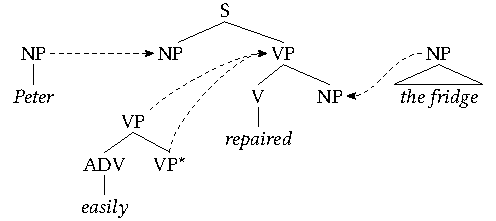
\includegraphics{graphics/abb51.pdf}
\caption{\label{fig-TAG-bsp1}Beispiel einer TAG-Ableitung des Satzes {\it Peter easily repaired the fridge}}
\end{figure}
Elementarbäume werden in \textsc{Initialbäume}\is{Initialbaum} und \textsc{Hilfsbäume}\is{Hilfsbaum} unterschieden, denen je eine eigene Verknüpfungsoperation zugeordnet ist, d.\,h.\ Initialbäume werden mittels \textsc{ Substitution}\is{Substitution} verknüpft, und Hilfsbäume mittels \textsc{Adjunktion}\is{Adjunktion}. Initialbäume und Hilfsbäume unterscheiden sich hinsichtlich ihrer Blätter: Nur Hilfsbäume verfügen über ein spezielles, mit einem Stern ($\ast$) versehenes Blatt, den sogenannten \textsc{Fu\ss knoten}\is{Fu\ss knoten}.  

\isi{Substitution} bedeutet die Ersetzung eines nicht-terminalen Blattes durch einen \isi{Initialbaum}. Ein Beispiel hierfür ist in Abbildung~\ref{fig-TAG-bsp1} dargestellt. Die Initialbäume {\it Peter} und {\it the fridge} ersetzen dort die nicht-terminalen Blätter von {\it repaired}. Dagegen versteht man unter \isi{Adjunktion} die Ersetzung eines Innenknotens durch einen Hilfsbaum. Der ursprünglich vom Innenknoten dominierte Teilbaum wird dann vom Fu\ss knoten dominiert. Dies ist in Abbildung~\ref{fig-TAG-bsp1} durch den Hilfsbaum {\it easily} exemplifiziert, der an den unteren VP-Knoten adjungiert wird. Die Adjunktion wird durch Adjunktionsbeschränkungen\is{Adjunktionsbeschränkung} geleitet, die es zulassen, für jeden Innenknoten \textsc{obligatorische Adjunktion (OA)}, \textsc{selektive Adjunktion (SA)} und \textsc{Null-Adjuntion (NA)} zu spezifizieren. Beispielsweise muss der tiefere VP-Knoten im {\it repaired}-Baum den {\it easily}-Hilfsbaum zur selektiven oder obligatorischen Adjunktion freigegeben haben. Ist dagegen kein Hilfsbaum zur selektiven Adjunktion zugelassen, spricht man von Null-Adjunktionsbeschrän\-kung. Einer weitverbreiteten Konvention entsprechend werden in dieser Arbeit die Blätter der Elementarbäume immer eine NA-Beschränkung\is{Adjunktionsbeschränkung} enthalten, falls nicht anders angezeigt.

Zwei wichtige Nebenprodukte der TAG-Ableitung sind der \textsc{abgeleitete Baum}\is{abgeleiteter Baum} und der \textsc{Ableitungsbaum}\is{Ableitungsbaum}. Sie sind für obiges Beispiel in Abbildung~\ref{fig-TAG-bsp2} wiedergegeben. Der Ableitungsbaum ist das Protokoll der Ableitung und charakterisiert den abgeleiteten Baum in eindeutiger Weise, indem seine Knoten Elementarbäume repräsentieren und seine Kanten Verknüpfungsoperationen. Die Kanten sind mit \textsc{Gorn-Adressen} beschriftet, die die \isi{Knotenadresse} (des Elementarbaums im Mutterknoten) anzeigen, an der eine Verknüpfung stattfand.\footnote{Die Gorn-Adresse\is{Gorn-Adresse} des Wurzelknotens ist das leere Wort $\varepsilon$. Die Gorn-Adresse des $i$-ten Kindes eines Knotens mit Gorn-Adresse $p$ ist $pi$. Gorn-Adressen sind benannt nach \cite{Gorn:67}.} Dabei gilt die Konvention, dass ein Mutterknoten den \textsc{Zielbaum}\is{Zielbaum} einer Verknüpfung darstellt, in dem ein nicht-terminaler Knoten durch den Elementarbaum des Tochterknotens ersetzt wurde. Im Beispiel gibt es nur einen Mutterknoten, {\tt repaired}, der den Elementarbaum des Verbs repräsentiert. Alle anderen Elementarbäume ersetzen durch Substitution oder Adjunktion einen Knoten von {\tt repaired}, sind also im Ableitungsbaum dessen Tochterknoten. Der Ableitungsbaum spielt eine wichtige Rolle bei der Berechnung der Semantik (siehe z.\,B.\ \citealt{Kallmeyer:Joshi:03,Kallmeyer:Romero:08}) und wird in Abschnitt \ref{sec-tag-ling} ausführlicher thematisiert.

\begin{figure}[t]
\centering
\begin{tabular}{cc}
Abgeleiteter Baum:\hspace*{3em} & Ableitungsbaum:\hspace*{4em} \\[2ex]
\begin{minipage}{17em}
\hspace{-1.5em}
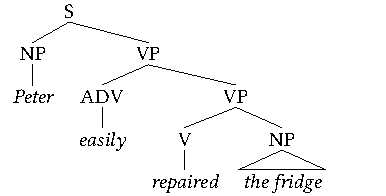
\includegraphics{graphics/abb52a.pdf}
\end{minipage}
&
\hspace{-2em}
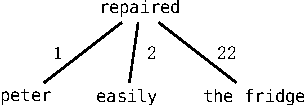
\includegraphics{graphics/abb52b.pdf}
\end{tabular}
\caption{\label{fig-TAG-bsp2}Beispiel für einen abgeleiteten Baum und einen Ableitungsbaum}
\end{figure}

\subsection{Gebräuchliche Varianten: LTAG, FSTAG und MCTAG}

Die sehr geraffte Darstellung bis hier entspricht etwa dem Kernverständnis des TAG"=Formalismus. Darauf aufbauend kursiert jedoch durch Erweiterungen oder Einschränkungen eine Unzahl von TAG-Varianten, von denen ich die Gebräuchlichsten ebenfalls kurz einführen möchte, nämlich LTAG, FSTAG und MCTAG.  

Die Elementarbäume in Abbildung~\ref{fig-TAG-bsp1} enthalten ein nicht-terminales Blatt, der auch \textsc{Anker} genannt wird. Eine TAG, die ausschlie\ss lich aus Elementarbäumen dieser Art besteht, wird \textsc{lexikalisierte TAG}\is{Lexicalized TAG (LTAG)} oder LTAG genannt. In dieser Arbeit werde ich die Termini TAG und LTAG synonym verwenden, da die Lexikalisierung von TAG bei der Modellierung natürlicher Sprache üblich ist, auch aus technischen Gründen (siehe \citealt{Schabes:etal:88, Schabes:90, Schabes:Joshi:90, Joshi:Schabes:91b}). Die umfangreichsten TAG-Implementierungen, \isi{XTAG} für das Englische \citep{xtag:01} und \isi{French TAG} für das Französische \citep{Abeille:02}, sind lexikalisiert. Ebenso die aus Baumbanken induzierten TAG \citep{Chiang:00,Xia:01,Chen:etal:06,Kaehammer:Demberg:12}.\footnote{\cite{Kaehammer:Demberg:12} induzieren neben der LTAG auch unlexikalisierte "`Prediction Trees"', um inkrementelle Ableitungen zu erhalten.}

Statt atomarer Knotenlabels benutzt man insbesondere bei Grammatiken mit großer Abdeckung (z.\,B.\ bei der XTAG-Grammatik) Merkmalsstrukturen\is{Merkmalsstruktur}. Diese TAG-Variante wird \textsc{FSTAG} oder \textsc{FTAG}\is{Feature-Structure-based TAG (FTAG)} (Feature-Structure-based TAG, \citealt{Vijay-Shanker:Joshi:88}) genannt und unterscheidet sich in der Ausdrucksstärke nicht von TAG, sofern die Menge der zulässigen Merkmalsstrukturen endlich ist.\footnote{Die Merkmalsstrukturen der FSTAG übernehmen die Funktion der Adjunktionsbeschränkungen\is{Adjunktionsbeschränkung} bei TAG.} Deshalb findet man in der TAG-Literatur selten den Terminus FSTAG und subsumiert ihn stillschweigend unter TAG -- so auch in dieser Arbeit. Die Merkmalsstrukturen\is{Merkmalsstruktur} in den Knoten bestehen jeweils aus zwei Blöcken, den \textsc{top}"=Merkmalen\is{top-Merkmal@\textsc{top}-Merkmal} und den  \textsc{bot(tom)}"=Merkmalen\is{bot-Merkmal@\textsc{bot(tom)}-Merkmal}, die bei der Verknüpfung von Elementarbäumen unterschiedlich behandelt werden. Bei der \isi{Substitution} werden die {\sc top}"=Merkmale des Zielblattes mit den {\sc top}-Merkmalen des Wurzelknotens des Initialbaums unifiziert. Abbildung~\ref{fig-tag-merkmal-1} soll dies veranschaulichen. Die {\sc bot}"=Merkmale des Zielblattes werden dabei ignoriert. Deshalb ist es üblicher, zu sagen, dass ein Substitutionsknoten keine {\sc bot}-Merkmale enthält. 
\begin{figure}[t]
\centering
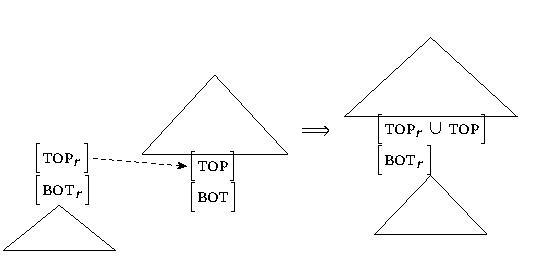
\includegraphics{graphics/abb53.pdf}
\caption{Schema der Merkmalsunifikation bei Substitution\label{fig-tag-merkmal-1}}
\end{figure}    
Das Verfahren bei \isi{Adjunktion} ist etwas komplizierter. Hier werden die {\sc top}-Merkmale des Wurzelknotens des Hilfsbaums mit den {\sc top}-Merkmalen des Zielknotens unifiziert, und die {\sc bot}-Merkmale des Fu\ss knotens mit den {\sc bot}-Merkmalen des Zielknotens. Schematisch ist dies in Abbildung~\ref{fig-tag-merkmal-2} dargestellt.
\begin{figure}[t]
\centering
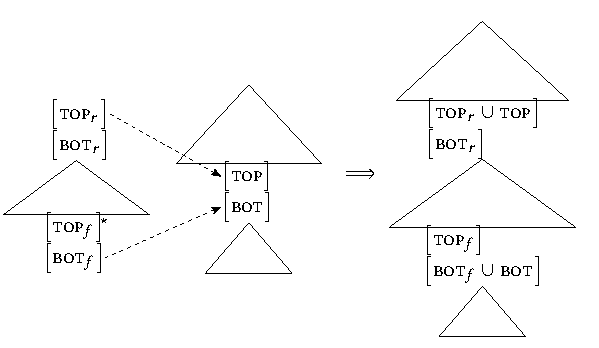
\includegraphics{graphics/abb54.pdf}
\caption{Schema der Merkmalsunifikation bei Adjunktion\label{fig-tag-merkmal-2}}
\end{figure}    
Nachdem die Verknüpfung der Elementarbäume abgeschlossen ist, werden zuletzt die {\sc top}-Merkmale und {\sc bot}"=Merkmale aller Knoten im abgeleiteten Baum unifiziert. 

Eine abweichende Form der Elementarstrukturen findet man in den TAG"=Varianten, die als \textsc{MCTAG}\is{Multi-Component TAG (MCTAG)} (Multi-Component TAG) bezeichnet und bereits bei \cite{Joshi:etal:75} als "`simultaneous TAG"' eingeführt werden. Die Elementarstrukturen können hier aus mehreren Elementarbäumen bestehen und beispielsweise Elementarbaummengen bilden. Eine Anwendung finden solche Elementarbaummengen  etwa bei der Simulation von Bewegungsanalysen\is{Bewegung} wie in Abbildung~\ref{fig-mctag-bsp}. Dort sind die \textit{wh}-bewegte NP und deren Spur in einer Elementarbaummenge gebündelt und können an unterschiedlichen Stellen im Zielbaum eingesetzt werden.  
\begin{figure}[t]
\centering
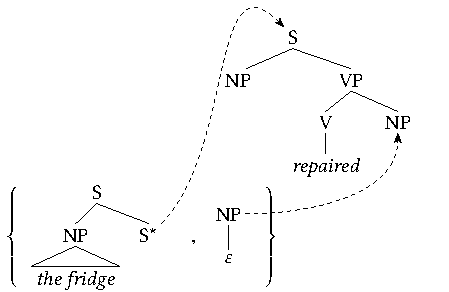
\includegraphics{graphics/abb55.pdf}
\caption{\label{fig-mctag-bsp}Beispiel einer Elementarbaummenge für \textit{wh}-Bewegung, die mit dem {\it repaired}-Elementarbaum verknüpft wird}
\end{figure}
An den Verknüpfungsoperationen sowie an der Form des abgeleiteten Baums und des Ableitungsbaums ändert sich nichts, zumindest nicht bei den klassischen MCTAG-Varianten\is{Multi-Component TAG (MCTAG)} von \cite{Weir:88}. Die Verwendung einer Elementarbaummenge ist jedoch zwei spezifischen Beschränkungen unterworfen: (i) alle Elemente einer Elementarbaummenge müssen bei der Ableitung berücksichtigt werden; (ii) die Verknüpfungsziele der Elemente einer Elementarbaummenge müssen sich im selben  Elementarbaum befinden, dann ist es eine \textsc{baumlokale MCTAG}\is{Multi-Component TAG (MCTAG)!baumlokale (TL-MCTAG)} oder \textsc{TL-MCTAG} wie in Abbildung~\ref{fig-mctag-bsp}, oder sie müssen mit den Elemente derselben Elementarbaummenge verknüpft werden, dann spricht man von einer \textsc{mengenlokale MCTAG}\is{Multi-Component TAG (MCTAG)!mengenlokale (SL-MCTAG)} oder \textsc{SL-MCTAG}. Ist das Verknüpfungsziel dagegen in dieser Hinsicht unbeschränkt, kann es also für die Elemente einer Elementarbaummenge in verschiedenen Elementarbaummengen liegen, spricht man von einer \textsc{nichtlokalen MCTAG}\is{Multi-Component TAG (MCTAG)!nichtlokale (NL-MCTAG)} oder \textsc{NL-MCTAG}. Weir zufolge ist die Verknüpfungslokalität von Elementarbaummengen einer NL-MCTAG nicht vollkommen unbeschränkt, denn die Elemente einer Elementar\-baummenge müssen simultan verwendet werden.\footnote{Die \isi{Simultanitätsbedingung} impliziert, dass die Elemente einer Baummenge einander im Ableitungsbaum nicht dominieren können, und dass die Baummengen im Ableitungsbaum nicht verschränkt sind. Für eine formale Darstellung der Simultanitätsbedingung siehe Kallmeyer (\citeyear[197]{Kallmeyer:05}; \citeyear[65f]{Kallmeyer:09}).} Das führt u.\,a.\ dazu, dass Elemente einer Elementarbaummenge nicht untereinander verknüpft werden können. Eine NL-MCTAG\is{Multi-Component TAG (MCTAG)!nichtlokale (NL-MCTAG)} ohne Simultanitätsbeschränkung hat \cite{Rambow:94} mit der Vector-MCTAG\is{Vector-MCTAG (V-TAG)} für die Modellierung kohärenter Konstruktion im Deutschen vorgeschlagen. Auf diese und andere MCTAG-Varianten gehen ich in Abschnitt \ref{sec-tag-varianten} und \ref{sec-ttmctag-formalismus} ausführlicher ein. 

\subsection{Ausdrucksstärke und Verarbeitungskomplexität}\is{schwache Kontextsensitivität|(}\label{sec:ausdrucksstaerke}

Eine wesentliche Motivation bei der Entwicklung von TAG ist es, einem Kompromiss zwischen Ausdrucksstärke und \isi{Verarbeitungskomplexität} zu entsprechen, für den \cite{Joshi:85} den Begriff der \textsc{schwachen Kontextsensitivität} (mild context"=sensitivity, MCS) prägte. Was die nötige Ausdrucksstärke für die Erfassung natürlicher Sprache betrifft, herrscht spätestens seit den Arbeiten von \cite{Huybrechts:84} und \cite{Shieber:85} Konsens darüber, dass kontextfreie Grammatiken\is{kontextfreie Grammatik} diesbezüglich nicht ausreichen. Als Beleg dafür dienen kreuzende Abhängigkeiten\is{kreuzende Abhängigkeit} im Niederländischen und Schweizerdeutschen, bei denen es sich um Valenzbeziehungen zwischen den Verben eines \isi{Verbalkomplex} und ihren nominalen Ergänzungen handelt. Shieber gibt das Beispiel in \ref{ex-shieber85-1}, wobei die Verbalfeldannotation und die Glossierung von mir stammt:

\exg. \label{ex-shieber85-1}\ldots mer {em Hans$^1$} {es huus$^2$} hälfed$^1$ aastriiche$^2$ \\
\ldots wir {dem Hans} {das Haus} helfen anstreichen {~}\\
\citep[(1)]{Shieber:85}

Aus \ref{ex-shieber85-1} lässt sich übrigens leicht ein VE-Satz\is{Satz!VE-} des Hochdeutschen formen, der ebenfalls eine kreuzende Abhängigkeit enthält:

\ex. dass wir das Haus$^2$ dem Hans$^1$ anstreichen$^2$ helfen$^1$

Da die vollständige Klasse der kontextsensitiven Sprachen weit über das erforderliche Ma\ss \ an Ausdrucksstärke hinausgeht und zudem eine zu hohe Verabeitungskomplexität aufweist, d.\,h.\ nicht polynomiell parsbar\is{polynomielle Parsebarkeit} ist, steht der Begriff der schwachen Kontextsensitivität für den Versuch, den für natürliche Sprachen nötigen Teilbereich innerhalb der polynomiell parsbaren Sprachen exakt zu definieren.  Einstweilen erfüllt eine schwach kontextsensitive Grammatik die folgenden Kriterien:\footnote{Als Kandidat für ein weiteres MCS-Kriterium wurde in letzter Zeit die Erzeugung von ausschlie\ss lich wohl-eingebetteten Abhängigkeiten diskutiert (siehe z.\,B.\ \citealt{Kuhlmann:Moehl:07, Kanazawa:09, Moennich:10}). Im Unterschied zur Erzeugung kreuzender Abhängigkeiten ist dies allerdings als Obergrenze der Ausdrucksstärke zu verstehen, d.\,h.\ nicht-wohleingebettete Strukturen sollen nicht erzeugt werden.}

\ex. \label{ex-kriterien-mcs} {\bf Kriterien der schwachen Kontextsensitivtät (MCS):}
\a.[(i)] Erzeugung mindestens aller kontextfreien Sprachen
\b.[(ii)] Erzeugung kreuzender Abhängigkeiten
\c.[(iii)] Konstantes Wachstum (oder Semi-Linearität)
\d.[(iv)] Polynomielle Parsebarkeit

Grob gesagt fordert das Kriterium des konstanten Wachstums\is{konstantes Wachstum} (oder der \isi{Semi-Linearität}), dass die Strings (oder "`Wörter"') einer MCS-Sprache durch Rekursion nur konstant "`wachsen"'. Das bedeutet, dass die Längen zweier Strings $w_i, w_j$ in einer MCS-Sprache maximal um ein beliebiges, konstantes $k$ differieren, falls es kein $w_x$ mit einer Länge zwischen der von $w_i$ und $w_j$  gibt. Anders ausgedrückt, falls $|w_i| < |w_j|$ und es gibt kein $w_x$, so dass $|w_i| < |w_x| < |w_j|$, dann gilt auch $|w_j| - |w_i| + n = k$, mit $1 \leq n \leq k$. Eine Folge des konstanten Wachstums ist beispielsweise, dass die Sprache $\{a^{2^n} | n \geq 1\}$ nicht erzeugt werden kann.

Die klassische TAG erfüllt die MCS-Kriterien und auch alle TAG"=Erweiterungen, die für die Sprachmodellierung eingesetzt werden, sollen sie erfüllen. Es ist z.\,B.\ bekannt, dass NL-MCTAG\is{Multi-Component TAG (MCTAG)!nichtlokale (NL-MCTAG)} das Kriterium der polynomiellen Parsebarkeit nicht erfüllt, Vector-MCTAG dagegen schon (siehe Abschnitt \ref{sec-tag-varianten-vtag}).    

Eine weitere wichtige Eigenschaft der Ausdrucksstärke von TAG ist die Möglichkeit, bestimmte CFGs, nämlich solche, die für jeden String immer nur endlich viele Ableitungen ermöglichen ("`finitely ambiguous"'), mit einer LTAG stark zu lexikalisieren (\citealt{Schabes:etal:88, Joshi:Schabes:91}). Lexikalisiert eine LTAG $G_{\mathit{LTAG}}$ eine CFG $G_{\mathit{CFG}}$ stark, dann generieren $G_{\mathit{LTAG}}$ und $G_{\mathit{CFG}}$ nicht nur dieselbe Stringsprache, sondern auch dieselbe Baumsprache.

Schlie\ss lich darf an dieser Stelle nicht der Hinweis fehlen, dass die Elementarbäume eine bezogen auf CFG-basierte Formalismen (CFG, HPSG, LFG) \textsc{erweiterte Lokalitätsdomäne}\is{erweiterte Lokalitätsdomäne} ("`extended domain of locality"') abbilden. Während eine CFG-Regel im Parsebaum einem Teilbaum der Höhe 1 entspricht und damit nur unmittelbare Dominanz ausdrücken kann, verfügen Elementarbäume über eine beliebige Höhe. Deshalb und dank der \textsc{Faktorisierung der Rekursion}\is{Faktorisierung der Rekursion} ("`factoring of recursion"') durch die Adjunktion von Hilfsbäumen ist es möglich, dass zwei Knoten aus demselben Elementarbaum im abgeleiteten Baum\is{abgeleiteter Baum} beliebig weit auseinanderliegen. Diese Mischung aus Lokalität in den Elementarbäumen und Nichtlokalität im abgeleiteten Baum ist ein wichtiger Ansatzpunkt für die Modellierung natürlicher Sprache mit TAG, zu der wir nun kommen. 
\is{Tree Adjoining Grammar (TAG)|)}\is{schwache Kontextsensitivität|)}


\section{TAG als linguistisches Framework} \label{sec-tag-ling}

Die Elementarbäume und Verknüpfungsoperationen einer TAG sind per se abstrakte mathematische Objekte, die zunächst einmal mit natürlicher Sprache nicht das Geringste zu tun haben. Damit sie als linguistisches Framework dienen können, müssen Elementarbäume und Verknüpfungsoperationen erst syntaxtheoretisch interpretiert werden, d.\,h.\ es muss erst festgelegt werden, welchen Entitäten der Syntaxtheorie sie wie entsprechen. Zusätzlich zu den Beschränkungen durch den Formalismus (z.\,B.\ Lexikalisierung) werden der Gestalt von Elementarbäumen deshalb auch linguistisch motivierte Wohlgeformtheitsbedingungen auferlegt. Erste Ansätze dazu gab es bei \cite{Abeille:88,Abeille:88b} und \cite{Frank:92}, die in jüngerer Zeit durch \cite{Abeille:Rambow:00} und \cite{Frank:02} präzisiert und erweitert wurden. Im Folgenden werde ich die syntaxorientierte Explikation der Wohlgeformtheitsbedingungen aus \cite{Frank:02} ausführlicher darstellen, aber auch die eher semantikorientierte Explikation aus \cite{Abeille:Rambow:00} am Ende des Abschnitts kurz erwähnen.%\\ 

\subsection{Allgemeine Wohlgeformtheitsbedingungen}

Eine erste, wichtige Idee, was ein Elementarbaum sein soll und was er enthalten soll, kommt bei \cite{Frank:02} mit der Fundamental TAG Hypothesis\is{Wohlgeformtheitsprinzip!Fundamental TAG Hypothesis} zum Ausdruck: 

\ex. {\bf Fundamental TAG Hypothesis (FTH)} \\
Every syntactic dependency is expressed locally within an elementary tree.
\citep[22]{Frank:02}

Zu den syntaktischen Abhängigkeiten zählen im Wesentlichen die Valenzbeziehungen, aber auch z.\,B.\ Bewegungsbeziehungen, d.\,h.\ die Beziehung zwischen einer bewegten Konstituente und seiner Spur, bis hin zur Beziehung zwischen extraponiertem Relativsatz und Antezedens \citep{Kroch:Joshi:87} und die \isi{Bindung} von Reflexiv- und Reziprokpronomen \citep{Ryant:Scheffler:06,Kallmeyer:Romero:07,Champollion:08}. Uns interessieren hier natürlich vor allem die Valenzbeziehungen. Diesbezüglich folgt aus der FTH übrigens nicht, dass der Valenzträger und alle valenzgebundenen Ko-Konstituenten in einem Elementarbaum repräsentiert sein müssen. Es ist vielmehr mit der FTH verträglich, dass jede \isi{Valenzbeziehung} durch einen eigenen Elementarbaum repräsentiert wird. 

Der \isi{Valenzträger} und seine \isi{Ergänzung} können im \isi{Elementarbaum} auf unterschiedliche Weise repräsentiert werden, nämlich 
\begin{itemize}
  \item durch lexikalische Anker, d.\,h.\ terminale Blätter,
  \item durch \isi{Substitutionsknoten} und \isi{Fu\ss knoten},
  \item durch Markierung eines Innenknotens\is{Innenknoten} für obligatorische Adjunktion.
\end{itemize}
Es ist nichts darüber ausgesagt, wie von diesen Repräsentationsweisen Gebrauch gemacht werden soll. Valenzträger und Ergänzung können also beliebig repräsentiert werden, wobei nur beachtet werden muss, dass die Elementarbäume lexikalisiert sind. Nicht ausgeschlossen ist also, dass die Ergänzung in einem Elementarbaum als lexikalischer Anker realisiert ist und der Valenzträger als Substitutionsknoten. Dies entspricht freilich nicht der üblichen Konvention, nach der die Repräsentation bzw.\ Realisierung des Valenzrahmens genau umgekehrt geschehen würde. Der Elementarbaum für {\it repaired} aus Abbildung~\ref{fig-TAG-bsp1}, der in Abbildung~\ref{fig-TAG-bsp1-1} nochmals wiedergegeben ist, befindet sich im Einklang mit dieser Konvention: Der Valenzträger ist der lexikalische Anker des Elementarbaums und seine Ergänzungen werden als nicht-terminale Blätter, d.\,h.\ hier als Substitionsknoten, repräsentiert. Man beachte, dass Frank in seinen Elementarbäumen eine andere Phrasenstruktur verwendet, worauf gleich noch eingegangen wird. Elementarbäume der Form in Abbildung~\ref{fig-TAG-bsp1-1} finden sich allerdings in der \isi{XTAG}-Grammatik \citep{xtag:01}. 
\begin{figure}[t]
\centering
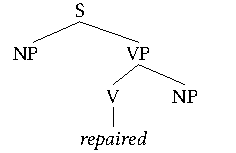
\includegraphics{graphics/abb56.pdf}
\caption{\label{fig-TAG-bsp1-1}Elementarbaum für {\it repaired}}
\end{figure}

Die in der FTH erwähnten syntaktischen Abhängigkeiten schlie\ss en auch nicht"=lokale oder weite Abhängigkeiten wie die \textit{wh}-Dislokation in \ref{ex-wh-dislocation} ein:

\ex. \label{ex-wh-dislocation}  (I wonder) [which book]$_i$ Gabriel had thought his friends should read $t_i$. \hfill \citep[25]{Frank:02}

Der Elementarbaum für {\it read} muss also auch direkt mit der \textit{wh}"=dislozierten Ergänzung {\it which book} verknüpft werden. In der \isi{XTAG}-Grammatik wird das mit dem zusätzlichen Elementarbaum in Abbildung~\ref{fig-TAG-bsp1-2} erreicht. 
\begin{figure}[t]
\centering
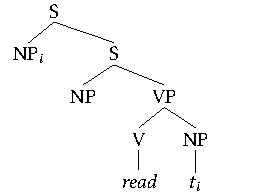
\includegraphics{graphics/abb57.pdf}
\caption{\label{fig-TAG-bsp1-2}Elementarbaum für {\it repaired} mit \textit{wh}-Bewegung}
\end{figure}
Die Dislokation in \ref{ex-wh-dislocation} kommt dann durch Substitution am höheren NP-Knoten (mit der Gorn-Adresse~1) zustande, während \textit{Gabriel had thought} durch Adjunktion am unteren S-Knoten eingefügt wird.

Der FTH zufolge sind also weite Abhängigkeiten wie die \textit{wh}-Dislokation\is{wh-Dislokation@\textit{wh}-Dislokation} in \ref{ex-wh-dislocation} Ergebnisse ein- oder mehrmaliger Adjunktion und lassen sich in einem Elementarbaum lokalisieren. Es gilt das folgende Korollar:

\ex. {\bf Non-local Dependency Corollary} \\
Non-local dependencies always reduce to local ones once recursion is factored away.
\citep[27]{Frank:02}

Die Lokalisierung von Dependenzbeziehungen\is{Dependenz} in einem Elementarbaum stellt folglich eine schwächere Form der Idealisierung der Kontinuität\is{Idealisierung!der Kontinuität} (siehe Abschnitt \ref{sec-strukturfrage}) dar, denn bestimmte Diskontinuitätstypen können in TAG durch Adjunktion direkt erzeugt werden. Diese Ausdrucksstärke aufgrund der erweiterten Lokalitätsdomäne fehlt beispielsweise CFG-basierten Grammatikformalismen, wo die Erzeugung von Diskontinuität allenfalls indirekt möglich ist (siehe Abschnitt~\ref{sec-ttmctag-modellierungsstrategien}). Dass jedoch nicht alle Diskontinuitätstypen mit TAG erzeugbar sind, wird sich unten in Abschnitt~\ref{sec-tag-grenzen} zeigen. %\\   


\subsection{Struktur und Kategorien der Innenknoten}

Die FTH und die Non-local Dependency Corollary lassen viele Aspekte eines Elementarbaums\is{Elementarbaum} unbestimmt: Wie sieht die Struktur eines Elementarbaums aus? Welche Dependenzbeziehungen werden zusammen in einem Elementarbaum repräsentiert? Und wie wird \isi{Dependenz} repräsentiert?  Um diese Fragen zu beantworten und eine der Konvention in Abbildung~\ref{fig-TAG-bsp1-1} und~\ref{fig-TAG-bsp1-2} nahekommende Gestalt der Elementarbäume zu erhalten, formuliert \cite{Frank:02} zwei weitere Wohlgeformtheitsbedingungen: die Condition on Elementary Tree Minimality (CETM)\is{Wohlgeformtheitsprinzip!CETM für TAG} und das $\theta$-Kriterium. 

Zunächst legt die CETM fest, welche Rolle der lexikalische Anker spielt und wie die Konfiguration und Beschriftung der \isi{Innenknoten} auszusehen hat:

\ex. {\bf Condition on Elementary Tree Minimality (CETM)} \label{ex-cetm} \\
The syntactic heads in an elementary tree and their projections must form the extended projection of a single lexical head.
\citep[54]{Frank:02}

Das hei\ss t zunächst einmal, dass ein Elementarbaum mindestens den lexikalischen Kopf bzw.\ den lexikalischen Anker und seine \isi{Projektion} enthält. Die Projektion eines lexikalischen Kopfs\is{Kopf} ist hier im Sinne des X-bar-Schemas\is{X-bar-Schema} \citep{Chomsky:70} zu verstehen, nämlich im Elementarbaum als Dominanzpfad über dem lexikalischen Kopf, für den gelten soll: Die morphosyntaktische Kategorie des lexikalischen Kopfs und der Knoten des Dominanzpfads sind im Wesentlichen identisch, abgesehen von der Annotation der Komplexitätsebene mit Strichen und dem Postfix P (für "`phrase"').\footnote{Zum X-bar-Schema siehe auch Abschnitt \ref{sec-strukturfrage}.} Sei also $X$ eine morphosyntaktische Kategorie eines lexikalischen Kopfs {\it head$_{\text{X}}$}, dann ist z.\,B.\ der Dominanzpfad $X\!P ~~ X' ~~ X$ eine mögliche Projektion von {\it head$_{\text{X}}$} mit dem syntaktischen Kopf $X$. Dementsprechend würden also Elementarbäume des Verbs \textit{reads} dem Schema in Abbildung~\ref{fig-cetm-1} folgen.
 
\begin{figure}[t]
\centering
\scalebox{0.9}{
\begin{forest}
sn edges
[VP [$\cdots$,triangle] [\phantom{$'$}V$'$ [$\cdots$,triangle] [V [\textit{reads}]] ]]
\end{forest}
}
%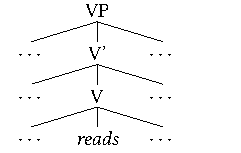
\includegraphics{graphics/abb58.pdf}
\caption{\label{fig-cetm-1}Schema einer X-bar-Projektion}
\end{figure}

Nun spricht Frank in der CETM-Formulierung in \ref{ex-cetm} jedoch von einer erweiterten Projektion ("`extended projection"'). Die \isi{erweiterte Projektion} \citep{Grimshaw:91,Grimshaw:00}  bezeichnet eine Erweiterung der X-bar-Projektion um funktionale, nicht-lexikalische Projektionen. Dazu zählen beispielsweise die Projektionen der syntaktischen Köpfe ("`syntactic heads"') C(omplemen\-tizer), I(nflection), T(ense) oder Neg(ative marker). Diese funktionalen syntaktischen Köpfe können funktionale Elemente wie Komplementierer (in C) oder Hilfsverben (in T) enthalten. Ein Verb wie {\it reads} lexikalisiert dann einen Elementarbaum entsprechend des Schemas in Abbildung~\ref{fig-cetm-2}.
\begin{figure}[t]
\centering
\scalebox{0.9}{
\begin{forest}
sn edges
[CP [$\cdots$,triangle]  
	[\phantom{$'$}C$'$ [C [$\cdots$]]
		[TP [$\cdots$,triangle] 
			[\phantom{$'$}T$'$ [T [$\cdots$]] 
				[VP [$\cdots$,triangle]
					[\phantom{$'$}V$'$ [$\cdots$,triangle]
						[V [\textit{reads}] ]
					]  
				] 
			] 
		] 
	] 
]
\end{forest}
}
% \Tree 
% [.CP [.C' C [.TP {\ldots} [.T' T [.VP [.V {\ldots} \textit{reads} {\ldots} ] ] {\ldots} ] {\ldots} ] {\ldots} ] {\ldots} ]
%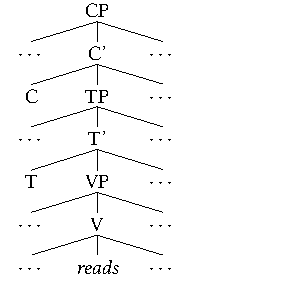
\includegraphics{graphics/abb59.pdf}
\caption{\label{fig-cetm-2}Schema einer erweiterte Projektion nach \citet[25]{Frank:02}}
\end{figure}
\citet[45ff]{Frank:02} argumentiert in Anlehnung an \cite{Grimshaw:91} und anderen für die Nützlichkeit der Annahme von erweiterten Projektionen im Rahmen der generativen Schule. Dessen ungeachtet werde ich im Weiteren X-bar-ähnliche Projektionen wie in Abbildung~\ref{fig-cetm-1} verwenden, die sich u.\,a.\ auch in den Elementarbäumen der XTAG-Grammatik wiederfinden. Die hier im Vordergrund stehende Idee des CETM ist also, dass ein Elementarbaum mindestens die Projektion des lexikalischen Kopfs im Sinne der X-bar-Theorie enthält, aber keine anderen syntaktischen Köpfe und deren Projektionen. Ich halte dies in der folgenden vereinfachten Formulierung des CETM fest:\is{Wohlgeformtheitsprinzip!CETM für TAG} 

\ex. \label{ex-cetm-vereinfacht} {\bf CETM} (vereinfacht) \\
Ein Elementarbaum enthält genau eine X-bar-Projektion, nämlich die des lexikalischen Kopfes.

Diese Vereinfachung des CETM, genauso wie Franks Originalformulierung, gilt auch für Elementarbäume von Modifizierern bzw.\ Angaben\is{Angabe}, die üblicherweise als \isi{Hilfsbaum} wie in Abbildung~\ref{fig-cetm-3} implementiert werden. Der vollständige Dominanzpfad über dem lexikalischen Kopf {\it easily} ist zwar $V\!P ~ A\!P ~ A$ und entspricht damit nicht der Projektion von {\it easily}, aber es gibt einen Dominanzpfad, nämlich $A\!P ~ A$, der dieses Kriterium erfüllt.\footnote{Frank betrachtet diesen Aspekt von Modifizierern natürlich vom Blickwinkel seiner Formulierung des CETM und ohne Bezug auf Dominanzpfade: 
\begin{quote}
Since the root VP node is not projected from a V head present in the elementary tree, the CETM is blind to its presence, just as phrasal argument slots do not count for the purposes of the CETM since they are not the projections of heads present in the elementary tree. \citep[63]{Frank:02}
\end{quote} 
Hier wird  der Unterschied zur CETM-Formulierung in \citet[54]{Frank:92} deutlich, wo noch eine Übereinstimmung von \isi{erweiterte Projektion} und \isi{Elementarbaum} gefordert wurde. Die Lizenzierung von modifizierenden Hilfsbäumen wie in Abbildung~\ref{fig-cetm-3}, wo der VP-Spine nicht zur erweiterten Projektion von \textit{easily} gehört, fällt dadurch schwerer (siehe \citealt[60f]{Frank:92}).} Ein deutlicher Unterschied zwischen den CETM-Versionen zeigt sich jedoch bei Komplementierern\is{Komplementierer} und Hilfsverben: Während Franks CETM\is{Wohlgeformtheitsprinzip!CETM für TAG} erlaubt, sie als \isi{Koanker} eines verbalen Kopfes zu behandeln, muss man für sie bei der vereinfachten CETM eigenständige Elementarbäume stipulieren. Letzteres entspricht auch dem Vorgehen in der \isi{XTAG}-Grammatik.  

\begin{figure}[t]
\centering
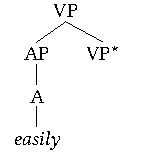
\includegraphics{graphics/abb510.pdf}
\caption{\label{fig-cetm-3}Hilfsbaum für den Modifizierer {\it easily}}
\end{figure}

Beide Versionen des CETM\is{Wohlgeformtheitsprinzip!CETM für TAG} erlauben also maximale Projektionen ohne syntaktischen Kopf, um bestimmte funktionale oder modifizierende Hilfsbäume zuzulassen. Man könnte sich damit zufrieden geben und alle sich daraus ergebenden Phrasenstrukturen akzeptieren. Man könnte jedoch stattdessen auch Vorsicht walten lassen und den abgeleiteten Baum phrasenstrukturell folgenderma\ss en restringieren:\is{Wohlgeformtheitsprinzip!Phrasenstrukturprinzip}  

\ex. {\bf Phrasenstrukturprinzip} \label{ex-psprinzip-1}\\
Der abgeleitete Baum\is{abgeleiteter Baum} enthält nur die vollständigen Projektionen der lexikalischen Anker.

Dadurch wird sichergestellt, dass die generierte Phrasenstruktur auch tatsächlich im Sinne des X-bar-Schemas\is{X-bar-Schema} wohlgeformt ist. Allein durch das CETM ist das nämlich nicht sichergestellt, wie wir z.\,B.\ in Abbildung~\ref{fig-extraposition-1} (S.~\pageref{fig-extraposition-1}) sehen werden. Außerdem bietet das Phrasenstrukturprinzip den Vorteil, die Bestandteile idiomatischer Mehrwortausdrücke\is{Mehrwortausdruck} als \isi{Koanker} eines Elementarbaums behandeln zu können, was z.\,B.\ von \cite{Abeille:Schabes:89,Abeille:Schabes:96} und \cite{Abeille:95} vorgeschlagen wird und dem CETM offensichtlich widerspricht \citep[Endnote~5, 292]{Frank:02}. Ich werde mich deshalb im Weiteren an das Phrasenstrukturprinzip\is{Wohlgeformtheitsprinzip!Phrasenstrukturprinzip} halten.


\subsection{Anzahl der Blätter}

Die abzweigenden Kanten und die daran hängenden nicht-terminalen Blätter werden bei \cite{Frank:02} durch eine TAG-Version des $\theta$-Kriteriums\is{theta-Kriterium@$\theta$-Kriterium} aus \cite{Chomsky:81} (siehe Abschnitt \ref{sec-existenzfrage}) lizenziert:\is{Wohlgeformtheitsprinzip!theta-Kriterium für TAG@$\theta$-Kriterium für TAG}

\ex. {\bf $\theta$-criterion (TAG version)} \label{ex-theta-criterion}
\a. If H is the lexical head of an elementary tree T, H assigns all of its $\theta$-roles in T.
\b. If A is a frontier non-terminal of elementary tree T, A must be assigned a $\theta$-role in T.
\z.
\citep[55]{Frank:02} 

Hierdurch wird analog zum $\theta$-Kriterium der \isi{GB-Theorie} ein bijektives Abbildungsverhältnis zwischen $\theta$-Rollen\is{theta-Rolle@$\theta$-Rolle} und nicht-terminalen Blättern innerhalb eines Elementarbaums erreicht. Es ist also sichergestellt, dass der \isi{Valenzträger} als lexikalischer Anker und alle seine Valenzrollen (bzw.\ seine semantischen Rollen\is{semantische Rolle}) als nicht-terminale Blätter repräsentiert werden. Der TAG-Formalismus stellt darüber hinaus die "`Füllung"' dieser nicht-terminalen Blätter im Verlauf der Ableitung sicher. Damit erbt das resultierende TAG-Modell die Idealisierungen, die in Abschnitt \ref{sec-valenzrealisierung} auf das $\theta$-Kriterium der GB-Theorie zurückgeführt wurden, nämlich die Idealisierung der Vollständigkeit\is{Idealisierung!der Vollständigkeit} und die Idealisierung der Funktionalität\is{Idealisierung!der Funktionalität}.

Das $\theta$-Kriterium\is{Wohlgeformtheitsprinzip!theta-Kriterium für TAG@$\theta$-Kriterium für TAG} für TAG geht jedoch noch weiter, indem es fordert, dass auch die \isi{Fu\ss knoten} in modifizierenden Hilfsbäumen wie oben in Abbildung~\ref{fig-cetm-3} eine $\theta$-Rolle tragen müssen. \citet[63f]{Frank:02} zufolge tun sie das auch, wobei dann jedoch keine $\theta$-Markierung, sondern eine $\theta$-Identifizierung\is{theta-Identifizierung@$\theta$-Identifizierung} ("`$\theta$-identification"') gemä\ss\ \citet[564]{Higginbotham:85} vorliegen soll. Unter einer $\theta$-Identifizierung versteht man die Mehrfachverwendung einer Variable in der semantischen Repräsentation, etwa die Mehrfachverwendung einer \isi{Eventvariable} \`a la Davidson wie in \ref{ex-thetacriterion-1}:

\ex. \label{ex-thetacriterion-1} {\tt $\exists$e [repaired(Peter,the fridge,e) $\wedge$ easily(e)]}

Dagegen soll die $\theta$-Markierung\is{theta-Markierung@$\theta$-Markierung} ein echtes Prädikat-Argument-Verhältnis voraussetzen.\footnote{Siehe auch die Diskussion im Zusammenhang mit der Darstellung der ARG-Beziehung\is{Valenzbeziehung!ARG} (S.~\pageref{sec-arg}ff).}

Was funktionale Hilfsbäume betrifft, die durch das vereinfachte CETM möglich geworden sind und deren lexikalische Anker über keine $\theta$-Rollen verfügen, ist eine Anpassung des $\theta$-Kriteriums nötig, welche in \ref{ex-valenzprinzip-tag} als Valenzprinzip\is{Wohlgeformtheitsprinzip!Valenzprinzip} vorgestellt werden wird. 

Eine Formulierung von Wohlgeformtheitsbedingungen für Elementarbäume unter Rückgriff auf deren Semantik findet man bei \citet[21f]{Abeille:Rambow:00}. Dabei wird naturgemä\ss \ die genaue Beschriftung der Knoten und die genaue Konfiguration der Elementarbäume offen gelassen. Die wesentlichen valenztheoretischen Annahmen decken sich jedoch mit denen der syntaktischen Wohlgeformtheitsbedingungen bei \cite{Frank:02}. Das Predicate Argument Co\-occurrence Principle (PACP)\is{Wohlgeformtheitsprinzip!PACP} etwa ist eine semantischere Formulierung des $\theta$-Kriteriums in der TAG-Version:\footnote{Das "`weak co-occurrence constraint"'und das "`strong co-occurrence constraint"' aus \cite{Joshi:Becker:Rambow:00} sind keine Beschränkungen auf den Elementarbäumen, sondern auf den Ableitungen. Siehe Abschnitt \ref{sec-tag-grenzen-scram}.} 

\ex. {\bf Predicate Argument Cooccurrence Principle (PACP)} \\
A predicative lexical item has (substitution or foot) nodes for each of its subcategorized arguments in its elementary trees. 

Wieder muss das Prädikat, d.\,h.\ der \isi{Valenzträger}, als lexikalischer Anker realisiert sein und mit seinen Argumenten in Form von nicht-terminalen Blättern innerhalb eines Elementarbaums kookkurrieren. Zudem wird explizit gemacht, dass alle Argumente in dieser Form angedeutet sein müssen. Im Unterschied zum $\theta$-Kriterium für TAG sind allerdings mehr nicht-terminale Blätter als Valenzrollen möglich, da keine Bijektion von Valenzrollen und Blättern gefordert wird. Au\ss erdem  besteht diese Bijektionsforderung nur für Elementarbäume mit prädikativem lexikalischen Anker, d.\,h.\ mit Valenzträger. Das PACP\is{Wohlgeformtheitsprinzip!PACP} verhindert also nicht, dass es Hilfsbäume mit nicht-prädikativen, funktionalen Ankern gibt.  

Solche Hilfsbäume mit funktionalen Ankern werden möglicherweise durch ein weiteres, allgemeineres Prinzip ausgeschlossen, das die semantische Minimalität der Elementarbäume fordert und das bei \cite{Abeille:Rambow:00} keinen Namen erhält:\footnote{Ähnlich \citet[5]{Kallmeyer:Romero:08} unter dem Begriff "`compositional minimality of elementary trees"': "`whenever the semantic contribution of an expression can be decomposed into the semantic contributions of different lexical items, each of these lexical items has a separate elementary tree."'}\is{Wohlgeformtheitsprinzip!NCSP}

\ex. {\bf Non-Compositional Semantics Principle (NCSP)} \\
An elementary tree is associated with some atomic (i.e., non-compositio\-nal) semantic meaning.

Das NCSP hat zum einen zur Folge, dass Elementarbäume nicht durch mehr als einen Valenzträger geankert werden dürfen (unabhängig davon, was genau unter den Begriff einer "`atomic semantic meaning"' fällt). Diese wichtige Einschränkung kommt oben in beiden CETM und auch im $\theta$-Kriterium für TAG zum Ausdruck. Zum anderen sortiert das NCSP solche Elementarbäume aus, die keine Bedeutung (bzw.\ "`semantic meaning"') beitragen. Davon betroffen sind Elementarbäume mit ausschließlich funktionalen Ankern wie dem \isi{Komplementierer} \textit{dass}. Im Folgenden wird dieser Aspekt des NCSP keine Rolle spielen. 

Die valenztheoretischen Implikationen der syntaktischen und semantischen Wohlgeformtheitsprinzipien für Elementarbäume sollen mithilfe der in Kapitel~\ref{ch-mit-valenz} etablierten Terminologie als Valenzprinzip reformuliert und zusammengefasst werden. Dabei wird auf eine Kompatibilität mit dem vereinfachten CETM in \ref{ex-cetm-vereinfacht} geachtet, d.\,h.\ auf eine Ermöglichung von Hilfsbäumen mit funktionalen Ankern.\is{Wohlgeformtheitsprinzip!Valenzprinzip}

\ex. {\bf Valenzprinzip (für TAG)} \label{ex-valenzprinzip-tag} \\
Lexikalisiert ein Valenzträger einen Elementarbaum, dann gilt: Es besteht ein bijektives Abbildungsverhältnis zwischen Valenzrollen einerseits und Substitutionsknoten und Fu\ss knoten andererseits.
% Elementarbäume entsprechen genau einem Valenzrahmen, wobei gilt:
% \a. Der lexikalische Anker ist der Valenzträger.
% \b. Es besteht ein bijektives Abbildungsverhältnis zwischen Valenzrollen einerseits und Substitutionsknoten und Fu\ss knoten andererseits.
% \c. Der Valenzrahmen ist vollständig repräsentiert. 

Lexikalisiert beispielsweise das Verb {\it reads} einen Elementarbaum $\gamma$ und verfügt der Valenzrahmen von {\it reads} über zwei Valenzrollen, dann bedingen diese dank des Valenzprinzips die Existenz genau zweier nicht-terminaler Blätter in $\gamma$. Lexikalisiert dagegen ein Komplementierer wie {\it that} ohne Valenzrahmen einen Elementarbaum, liegt das außerhalb des Geltungsbereichs des Valenzprinzips.
  
Das Valenzprinzip\is{Wohlgeformtheitsprinzip!Valenzprinzip} führt also wie das $\theta$-Kriterium und das PACP zur Idealisierung der Vollständigkeit\is{Idealisierung!der Vollständigkeit} und zur Idealisierung der Funktionalität\is{Idealisierung!der Funktionalität}. Außerdem unterscheidet das Valenzprinzip ebenfalls nicht zwischen obligatorischen und fakultativen Ergänzungen\is{Ergänzung}. Der wesentliche Unterschied besteht darin, dass beim Valenzprinzip obligatorische und fakultative Ergänzungen nicht in jedem Elementarbaum repräsentiert sein müssen, dass \textit{reads} also bei gleichem Rolleninventar unterschiedliche Valenzrahmen haben kann. Mit dem Valenzprinzip gibt es daher die Wahl zwischen zwei Modellierungsansätzen: Zum einen kann man {\it reads} einen eindeutigen Valenzrahmen zuweisen. Dann muss ein zusätzlicher Mechanismus, z.\,B.\ in Form von phonetisch leeren Elementarbäumen, bereitstehen, durch den die Realisierung der fakultativen Ergänzungen\is{Ergänzung!fakultative} zumindest oberflächlich umgangen werden kann, denn der Elementarbaum von \textit{reads} muss ja qua Valenzprinzip die nicht-terminalen Blätter für fakultative Ergänzungen enthalten. Dieser Ansatz verhält sich analog zum Ansatz der \isi{GB-Theorie} mit der dort vertretenen \isi{Schnittstellenuniformität} (siehe Abschnitt~\ref{sec-existenzfrage}). Und diesen Ansatz verfolgt auch Frank, indem er am Projektionsprinzip der GB-Theorie anknüpft \citep[64]{Frank:02}. Darüber hinaus erlaubt das Valenzprinzip\is{Wohlgeformtheitsprinzip!Valenzprinzip} aber auch, einem Valenzträger mehrere Valenzrahmen zuzuweisen, z.\,B.\ bei \textit{reads} mit und ohne Akkusativ-Ergänzung, und damit auch die entsprechenden Elementarbäume. Auf leere Kategorien\is{leere Kategorie} für die Modellierung von fakultativen Ergänzungen\is{Ergänzung!fakultative} kann dann verzichtet werden. Die Multiplizierung der Valenzrahmen wird beispielsweise von \cite{Jacobs:94a} vorgeschlagen. Dieser zweite Ansatz steht beim $\theta$-Kriterium\is{Wohlgeformtheitsprinzip!theta-Kriterium für TAG@$\theta$-Kriterium für TAG} und beim PACP\is{Wohlgeformtheitsprinzip!PACP} deswegen nicht zur Verfügung, weil dort das Inventar der semantischen Rollen\is{semantische Rolle} (nicht der Valenzrollen) bijektiv auf syntaktische Positionen abgebildet wird.





\subsection{Substitution oder Adjunktion?} \label{sec-ableitungsbaum}\is{Substitution|(}\is{Adjunktion|(}

Das Valenzprinzip\is{Wohlgeformtheitsprinzip!Valenzprinzip} lässt offen, ob Valenzträger mit Ergänzungen per Substitution oder Adjunktion verknüpft werden. Es wäre natürlich wünschenswert, wenn sich der Unterschied zwischen \isi{Ergänzung} und \isi{Angabe} in der Art der Verknüpfungsoperation manifestierte, indem etwa Ergänzungen immer substituieren und Angaben immer adjungieren. Doch das lässt sich leider nicht durchhalten, da es in manchen Konfigurationen für das Adjungieren des Valenzträgers an die Ergänzungen keine Alternative gibt. Ummantelt nämlich die Ergänzung den Valenzträger, wie in Abbildung~\ref{fig-TAG-raising} die Satzergänzung {\it Peter to sleep} das Anhebungsverb\is{Anhebung} {\it seems}, dann kann dies im Geltungsbereich des Valenzprinzips nur per Adjunktion generiert werden. Au\ss er bei Anhebungsverben trifft man auf eine solche Valenzträgerummantelung bzw.\ ein solches Ergänzungssplitting auch bei Hilfs-\is{Hilfsverb} und Modalverben\is{Modalverb} und bei Brückenverben\is{Brückenkonstruktion}.

\begin{figure}[t]
\centering
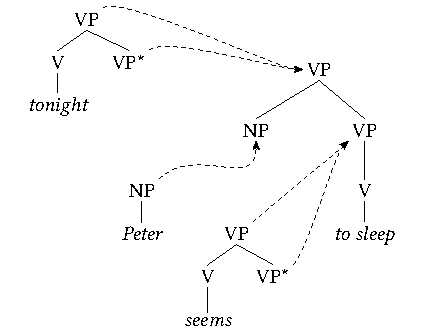
\includegraphics{graphics/abb511.pdf}
\caption{\label{fig-TAG-raising}Derivation einer Anhebungskonstruktion}
\end{figure}

Das Valenzverhältnis zwischen \isi{Hilfsbaum} und \isi{Zielbaum} ist also uneinheitlich: Der Hilfsbaum ist mal der Valenzträger, mal eine Angabe. Wenn aber im Ableitungsbaum adjungierte und substituierte Elementarbäume gleicherma\ss en vom Zielbaum dominiert werden, wie in Abbildung~\ref{fig-TAG-raising2} dargestellt, dann führt das bei Anhebungskonstruktionen zu einer falschen dependenziellen\is{Dependenz} Repräsentation, bei der die Satzergänzung den Valenzträger regiert.\footnote{Darüber hinaus können Dependenzbeziehungen\is{Dependenz} im Ableitungsbaum fehlen \citep{Rambow:etal:95}.}
\begin{figure}[t]
\centering
\begin{tabular}{cc}
Ableitungsbaum: & Dependenzgraph: \\[2ex]
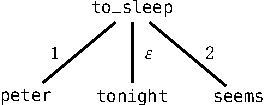
\includegraphics{graphics/abb512a.pdf}
&
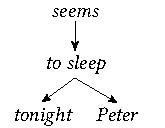
\includegraphics{graphics/abb512b.pdf}
\end{tabular}
\caption{\label{fig-TAG-raising2}Diskrepanz zwischen Ableitungsbaum und Dependenzgraph}
\end{figure} 
Ändert man dagegen die Darstellung der Adjunktion im Ableitungsbaum so, dass Hilfsbäume nun die Zielbäume dominieren, dominieren nicht nur Anhebungsverben ihre Satzergänzungen, sondern auch Angaben den Valenzträger. Man erhält also einen mehrwurzligen Ableitungsgraphen\is{Ableitungsbaum} wie in Abbildung~\ref{fig-TAG-raising3}.
\begin{figure}[t]
\centering
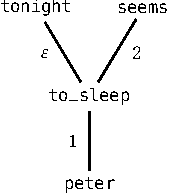
\includegraphics{graphics/abb513.pdf}
\caption{\label{fig-TAG-raising3}Mehrwurzliger Ableitungsgraph mit invertierten Adjunk"-tions"-kanten}
\end{figure} 
Abgesehen davon, dass mehrwurzlige Dependenzgraphen in der Dependenztheorie kaum Verwendung finden, entspricht dieser Ableitungsgraph auch nicht dem dependenziellen Verständnis der Valenzträger-Angabe-Relation. Es besteht also eine fundamentale Diskrepanz zwischen TAG-Ableitungsbaum und klassischem Dependenzgraphen. Will man trotzdem eine dependenzartigere Struktur des Ableitungsbaums erreichen, muss man erhebliche Änderungen am TAG-Formalismus oder am Valenzprinzip vornehmen \citep{Rambow:etal:95,Schabes:Shieber:94}.            

Die Indifferenz der Adjunktion hinsichtlich Komplementation und Modifikation ist letztlich eine Folge der konsequenten Anwendung des Valenzprinzips\is{Wohlgeformtheitsprinzip!Valenzprinzip}, das ja semantische Beziehungen (d.\,h.\ Prädikat-Argument-Beziehungen oder Mehrfachverwendungen einer Variable) zwischen lexikalischem Anker und nicht"=terminalen Blättern in den Vordergrund rückt. Folglich sollte man vielleicht den \isi{Ableitungsbaum} nicht als missglückten Dependenzgraphen begreifen, sondern  im weiteren Sinne als semantischen Graphen, wie das \cite{Candito:Kahane:98} vorschlagen. Dann stört es nicht, die Adjunktionen im Ableitungsbaum generell so zu repräsentieren, dass ein Hilfsbaum den Zielbaum dominiert.
\is{Substitution|)}\is{Adjunktion|)}


\subsection{Ökonomieprinzip}

Abschlie\ss end möchte ich eine Wohlgeformtheitsbedingung ganz anderer, nicht"=linguistischer Art formulieren, der die Rolle eines Ockham'schen Rasiermessers für TAG-Grammatiken zukommt:\is{Wohlgeformtheitsprinzip!Oekonomieprinzip@Ökonomieprinzip} 

\ex. {\bf Ökonomieprinzip}\label{ex-oekonomieprinzip-tag} \\
Die Elementarbäume sind so geformt, dass die Anzahl und die Grö\ss e der Elementarbäume minimal ist.     

Das Ökonomieprinzip wendet sich beispielsweise gegen die Existenz von Hilfsbäumen, die nirgendwo adjungieren können, oder gegen die Existenz von internen Knoten, an die nicht adjungiert werden kann. Mir ist klar, dass das Ökonomieprinzip, abgesehen vielleicht von solchen einfachen Beispielen, hochproblematisch ist, denn zum einen ist das Prädikat "`minimal"' hier nicht verifizierbar (dafür müsste man nämlich alle möglichen Grammatiken in Betracht ziehen, von denen es unendlich viele gibt) und zum anderen ist nicht ausgeschlossen, dass es mit anderen Wohlgeformtheitsbedingungen wie dem CETM konfligiert. Zumindest das Konfliktpotential lässt sich jedoch mühelos eliminieren, indem das Ökonomieprinzip nachgeordnet bzw.\ als Metaprinzip behandelt wird.\footnote{Freilich erspart dieser Schritt nicht das Nachdenken über Fälle, in denen die Ökonomie in eine andere Richtung weist als stipulierte, linguistische Wohlgeformtheitsbedingungen.} Und auch wenn sich die Minimalität prinzipiell nicht verifizieren lässt, ist sie doch ein wichtiges Ideal bei der Implementierung und Gegenüberstellung von Grammatiktheorien.     


\section{Die Grenzen von TAG} \label{sec-tag-grenzen}

In diesem Abschnitt betrachten wir die Grenzen der \isi{Ausdrucksstärke} von TAG unter dem Einfluss der gerade dargestellten Wohlgeformtheitsbedingungen\is{Wohlgeformtheitsprinzip}.\footnote{Siehe auch \citet[Abschnitt~2.4]{Gerdes:02b}, wo die Grenzen von TAG ebenfalls mit Blick auf die Modellierung des Deutschen dargestellt werden.} Im Mittelpunkt steht also die linguistische oder \textsc{derivationelle Mächtigkeit}\is{derivationelle Mächtigkeit}  \citep{Becker:Rambow:Niv:92} des TAG-Formalis\-mus.\footnote{Man könnte hier auch die etwas allgemeinere Generative Attachment Capacity \citep{Kallmeyer:06} in Betracht ziehen.} Die derivationelle Mächtigkeit unterscheidet sich von der generativen Mächtigkeit\is{generative Mächtigkeit} durch den Bezug auf die Formatierung der Elementarstrukturen. Es wird also berücksichtigt, wie Strukturen erzeugt werden, und nicht nur die erzeugte Struktur selber betrachtet.\footnote{Ein Kriterium für MCS\is{schwache Kontextsensitivität} ist die Erzeugung kreuzender Abhängigkeiten\is{kreuzende Abhängigkeit}. Ist dies nun eine Eigenschaft der derivationellen oder der generativen Mächtigkeit? Man kann möglicherweise beides sehen, abhängig von der zugrundegelegten formalen Sprachklasse: Bei der \isi{Zählsprache} $\{a^n ~ b^n | n \in \mathbb{N}\}$ ist das eine Eigenschaft der derivationellen Mächtigkeit, denn es wird zusätzliche eine bestimmte Ko-Indizierung verlangt, die in der Sprache selber nicht sichtbar ist; bei der Zählsprache $\{a^n ~ b^m ~ c^n ~ d^m | n,m \in \mathbb{N}\}$ und der \isi{Kopiersprache} $\{ww|w\in\{a,b\}^*\}$ ist es dagegen eine Eigenschaft der generativen Mächtigkeit, denn die Ko-Indizierung ist hier quasi Teil der Sprache. Bei den natürlichen Sprachen gehört etwa das Niederländische zur ersten Klasse und das Schweizerdeutsche zur zweiten. Siehe Beispiel~\ref{ex-shieber85-1} und die Diskussion in \cite{Shieber:85}.} 

\subsection{Scrambling bei kohärenten Konstruktionen} \label{sec-tag-grenzen-scram}

Aus Sicht der generativen Mächtigkeit\is{generative Mächtigkeit} ist das \isi{Scrambling} bei kohärenten Konstruktionen\is{kohärente Konstruktion} keine Herausforderung. Das String-Schema bei Verbletzt"=Sätzen \linebreak stellt sich folgenderma\ss en dar:

\ex. $\mathit{NP}^n ~~ V^m$

Einer Anzahl von NPs folgt also eine Anzahl von Vs. Dieses String-Schema übergeht jedoch die Valenzrelationen zwischen NPs und Vs, die qua Valenzprinzip\is{Wohlgeformtheitsprinzip!Valenzprinzip} die Elementarstrukturen einschränken. Ich nehme im Folgenden an, dass die NP-Wörter des String-Schemas den NP-Substitutionsknoten der Elementarbäume entsprechen, die von V lexikalisiert werden. Ein String-Schema ist dann, bezogen auf die dahinterstehenden Elementarbäume, eine Mischung aus nicht-terminalen NPs und terminalen Vs. Tatsächlich interessant ist also ein String-Schema wie in \ref{ex-schema0}, in dem die Wörter so mit Indizes ($i,j,k,l$) annotiert sind, dass Wörter mit identischem Index aus derselben Elementarstrukturinstanz stammen:\footnote{Indizierte Sprachen und der Begriff der derivationellen Mächtigkeit\is{derivationelle Mächtigkeit} werden in \cite{Becker:Rambow:Niv:92} formal eingeführt. Siehe auch \citet[41]{Rambow:94}.}

\ex. $\mathit{NP}_i \ldots \mathit{NP}_j ~~ V_k \ldots V_l$ \label{ex-schema0}   

Das  Valenzprinzip\is{Wohlgeformtheitsprinzip!Valenzprinzip} zusammen mit dieser Indizierung entspricht dem, was \citet[175]{Joshi:Becker:Rambow:00} das \textsc{Weak Co-occurrence Constraint (WCC)}\is{Weak Co-occurrence Constraint (WCC)} nennen. Sollen darüber hinaus die  Verben so verknüpft werden, dass der Elementarbaum von $V_i$ immer an den Elementarbaum von $V_{i+1}$ adjungiert, dann ist \citet[177]{Joshi:Becker:Rambow:00} zufolge das \textsc{Strong Co-occurrence Constraint (SCC)}\is{Strong Co-occurrence Constraint (SCC)} erfüllt.\footnote{\label{fn-wcc-scc}WCC und SCC fu\ss en auf dem "`Co-occurrence Constraint"', einer Art Valenzprinzip (siehe auch \citealt[22]{Becker:Joshi:Rambow:91}): "`We are really only interested in linguistically appropriate grammars, namely those that exploit the extended domain of locality and whose trees obey the constraint that each elementary tree encapsulates the lexical anchor and positions for all of its arguments and no other arguments."' \citep[175]{Joshi:Becker:Rambow:00}} %\\

\cite{Becker:Joshi:Rambow:91} zeigen nun, dass TAG nicht die \isi{derivationelle Mächtigkeit} besitzt, um das folgende String-Schema der Indizierung entsprechend zu erzeugen:

\ex. $\mathit{NP}_2 ~ \mathit{NP}_1 ~ \mathit{NP}_2 ~ \mathit{NP}_1 ~ V_2 ~ V_1$ \label{ex-schema1}

Der Grund dafür ist recht offensichtlich: Da \ref{ex-schema1} aus zwei Elementarbäumen abgeleitet werden muss, nämlich aus einem über dem String $\mathit{NP}_1 ~ \mathit{NP}_1 ~ V_1$ und aus einem über den String $\mathit{NP}_2 ~ \mathit{NP}_2 ~ V_2$, führt deren Verknüpfung zu sechs Teilstrings. Die Adjunktionsoperation des TAG-Formalismus kann jedoch maximal fünf Teilstrings erzeugen. Sätze wie \ref{ex-schema1-bsp} sind also allein mit TAG nicht zu bewältigen, wenn ein Valenzrahmen vollständig in einem \isi{Elementarbaum} realisiert wird:

\ex. da\ss \ des Verbrechens der Detektiv den Verdächtigen dem Klienten zu überführen versprochen hat \hfill\label{ex-schema1-bsp}\mbox{\citep[(2b)]{Becker:Joshi:Rambow:91}}

Ein Beispiel etwas anderer Art findet sich bei \cite{Rambow:94}:

\exg. {Dieses Buch} hat {den Kindern} niemand {zu geben} versucht.  \\
$\mathit{NP}_2$ $V_1$ $\mathit{NP}_2$ $\mathit{NP}_1$ $V_2$ $V_1$ \\
\citep[42]{Rambow:94} \label{ex-schema2}

Anders als in \ref{ex-schema1-bsp} liegt hier ein Verbzweit-Satz\is{Satz!V2-} vor. Damit das Beispiel funktioniert, muss das finite \isi{Hilfsverb} zusammen mit dem regierten Vollverb {\it versucht} und der Nominativ-NP in einem Elementarbaum realisiert sein. Diese Bündelung ist nicht ohne Alternative, denn das finite Hilfsverb könnte auch vom infiniten Vollverb und dem \isi{Subjekt} getrennt und durch einen eigenen Elementarbaum repräsentiert werden. 

Doch selbst wenn es technisch möglich ist, fünf Teilstrings durch die Adjunktionsoperation zu erzeugen, stehen die involvierten Elementarbäume nicht immer im Einklang mit dem Valenzprinzip\is{Wohlgeformtheitsprinzip!Valenzprinzip}. So können das String-Schema in \ref{ex-schema1} und der Satz \ref{ex-schema1-bsp} zwar zu \ref{ex-schema21} vereinfacht werden: 

\exg. dass {der Detektiv} {den Verdächtigen} {dem Klienten} {zu überführen} {versprochen hat}  \\
$~$ $\mathit{NP}_1$ $\mathit{NP}_2$ $\mathit{NP}_1$ $V_2$ $V_1$ \\
\label{ex-schema21}

Aber dann muss der Elementarbaum des eingebetteten Verbs $V_2$ an den Elementarbaum des regierenden Verbs $V_1$ adjungieren -- anders ist eine Erzeugung von fünf Teilstrings nicht zu schaffen. Das ist mit dem Valenzprinzip jedoch unvereinbar, da der Elementarbaum von $V_2$ einen \isi{Fu\ss knoten} zuviel bzw.\ der Elementarbaum von $V_1$ einen Fu\ss knoten zuwenig hat.  %\\

\cite{Becker:Joshi:Rambow:91} und \cite{Joshi:Becker:Rambow:00} betrachten auch String-Schemata, in denen jedes Verb genau eine Nominalphrase regiert, die also Wörter der indizierte Scramblingsprache $\scrind$\is{indizierte Scramblingsprache ($\scrind$)} sind:\footnote{\citet[200]{Kallmeyer:05} bemängelt an  $\scrind$, dass damit nicht alle Scrambling-Möglichkeiten im Deutschen erfasst sind. Auf die von ihr vorgeschlagene Variante trifft dies jedoch auch nicht zu, da diese etwa Oberfeldumstellungen\is{Verbalkomplex!Oberfeldumstellung} oder partielle Voranstellungen\is{Voranstellung!partielle} nicht abdeckt. Man sollte $\scrind$ also besser als Abstraktion über einen aussagekräftigen Teilbereich des Kohärenzphänomens betrachten, die sich als Messlatte für die derivationelle Mächtigkeit von TAG-Varianten eignet.}

\ex. $\scrind = \{ \sigma(\mathit{NP}_1,\ldots,\mathit{NP}_m) V_m \ldots V_1 | m \geq 1$ and $\sigma$ ist eine Permuta\-tion$\}$ 

Im Gültigkeitsbereich des WCC\is{Weak Co-occurrence Constraint (WCC)} soll TAG in der Lage sein, alle Scramblingmöglichkeiten bei Verbalkomplexen\is{Verbalkomplex} mit maximal vier Verben zu erzeugen (\citealt[23]{Becker:Joshi:Rambow:91}; \citealt[177]{Joshi:Becker:Rambow:00}), also die Menge $\{ \sigma(\mathit{NP}_1, \ldots, \mathit{NP}_k) V_k \ldots$ $V_1 | k \leq 4, \sigma$ ist eine Permuta\-tion$\}$. Ich bezweifle allerdings, ob das stimmt.\footnote{Leider wird der Beweis in \citet{Becker:Joshi:Rambow:91} und \citet{Joshi:Becker:Rambow:00} nicht mitgeliefert, sondern auf ein unveröffentlichtes, unauf"|findbares Manuskript von Tilman Becker und Owen Rambow verwiesen, das diesen enthalten soll. Es wird nur angedeutet, dass für das Unvermögen, Scrambling bei Verbalkomplexen $> 4$ korrekt zu erfassen, das String-Schema $\mathit{NP}_3 ~ \mathit{NP}_1 ~ \mathit{NP}_5 ~ \mathit{NP}_2 ~ \mathit{NP}_4 ~ V_5 ~ V_4 ~ V_3 ~ V_2 ~ V_1$ verantwortlich sei.  Vermutlich ist hier das Problem, dass der Elementarbaum von $\mathit{NP}_2 V_2$ zweimal adjungieren müsste, was TAG ausschlie\ss t.} Tatsächlich fangen die Probleme schon bei Verbalkomplexen\is{Verbalkomplex} mit drei Verben an, nämlich bei folgendem String-Schema:

\ex. $\mathit{NP}_2 ~ \mathit{NP}_3 ~ \mathit{NP}_1 ~ V_3 ~ V_2 ~ V_1$\label{ex-schema-231} 

Bei der Erzeugung dieses String-Schemas mit einer TAG scheint es mir unvermeidbar, dass das tiefste Verbs $V_3$ am höchsten Verb $V_1$ adjungiert. Mit Blick auf das WCC\is{Weak Co-occurrence Constraint (WCC)} (bzw.\ das Valenzprinzip) hat der Elementarbaum von $V_3$ also in jedem Fall einen Fu\ss knoten zuviel. Auch \citet[(6)]{Joshi:Becker:Rambow:00} erwähnen das String-Schema in \ref{ex-schema-231} -- nur leider nicht im Zusammenhang mit dem WCC, sondern mit dem SCC\is{Strong Co-occurrence Constraint (SCC)}. Der Grund dafür liegt vermutlich darin, dass \cite{Joshi:Becker:Rambow:00} an dieser Stelle nur auf die Indizierung achten und nicht wie angekündigt (siehe oben) auch auf das Valenzprinzip. Indem das SCC\is{Strong Co-occurrence Constraint (SCC)} -- anders als das WCC -- auch die Indizierung des Verbalkomplex auswertet, wird dem Valenzprinzip\is{Wohlgeformtheitsprinzip!Valenzprinzip} implizit Rechnung getragen. Bezogen auf deren Definition sind aber sowohl das SCC als auch das WCC zu stark für die Derivation von \ref{ex-schema-231}. Beide können somit alle Scramblingmöglichkeiten nur bei Verbalkomplexen mit zwei Verben derivieren, also die Menge $\{ \sigma(\mathit{NP}_1,\ldots,\mathit{NP}_k) V_k \ldots V_1 | k \leq 2, \sigma$ ist eine Permuta\-tion$\}$.

Natürlich könnte es sein, dass \cite{Joshi:Becker:Rambow:00} die Definition des WCC\is{Weak Co-occurrence Constraint (WCC)} anders intendiert haben als oben festgelegt. Ich halte das aber für unwahrscheinlich, denn sie stellen ihre Arbeit explizit in den Geltungsbreich des Valenzprinzips (bzw.\ des "`co-occurrence constraint"').\footnote{Siehe Fu\ss note~\ref{fn-wcc-scc}.} Andernfalls wäre das WCC für die linguistische Modellierung uninteressant. Au\ss erdem gibt es bei anderen String-Schemata tatsächlich einen Unterschied zwischen WCC und SCC\is{Strong Co-occurrence Constraint (SCC)}, was sich z.\,B.\ mit folgendem String-Schema belegen lässt:    

\ex. $\mathit{NP}_1 ~ \mathit{NP}_3 ~ \mathit{NP}_2 ~ V_3 ~ V_2 ~ V_1$\label{ex-schema-132}

Dieses String-Schema kann mittels der Grammatik in Abbildung~\ref{fig-schema-132} deriviert werden, die dem WCC genügt, jedoch nicht dem SCC. Eine entsprechende Grammatik mit SCC scheint mir dagegen nicht konstruierbar.
\begin{figure}[t]
\centering
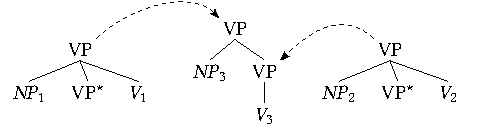
\includegraphics{graphics/abb514.pdf}
\caption{\label{fig-schema-132}Derivation des String-Schemas $\mathit{NP}_1 ~ \mathit{NP}_3 ~ \mathit{NP}_2 ~ V_3 ~ V_2 ~ V_1$, die dem WCC genügt, jedoch nicht dem  SCC}
\end{figure}

Missverständlich ist auch das in der Einleitung von \cite{Joshi:Becker:Rambow:00} vorgegriffene Fazit, dass LTAG nicht in der Lage sei, \isi{Long Distance Scrambling (LDS)} aus Einbettungen der Tiefe $>2$, d.\,h.\ kohärente Verbalkomplexe\is{Verbalkomplex} mit drei Verben, adäquat zu beschreiben.\footnote{"`We show that in the case of scrambling we are able to find a class of LTAG which have the property that as a class they are adequat [\ldots] to describe scrambling from up to two levels of embedding, and beyond two levels they fail."' \citep[167]{Joshi:Becker:Rambow:00}} Die maximale Einbettungstiefe ist tatsächlich abhängig von der Anzahl der Ergänzungen pro Verb. Wie wir in \ref{ex-schema1} sehen können, reicht bei zwei Ergänzungen pro Verb bereits eine Einbettungstiefe von $1$ aus, um mit TAG nicht immer adäquat beschreibbar zu sein. Andererseits sind auch kohärente Konstruktionen\is{kohärente Konstruktion} mit einer Einbettungstiefe $>2$ denkbar, die kein Problem für TAG darstellen:\footnote{Das Schema in \ref{ex-schema3} wird von \citet[190]{Kallmeyer:05} irrtümlicherweise als in diesem Sinne problematisch für LTAG bezeichnet. Der Grund ist wohl das angesprochene, missverständliche Fazit aus \citet[167]{Joshi:Becker:Rambow:00}.} 

\exg. dass {den Kühlschrank} niemand {zu reparieren} {zu versuchen} {zu versprechen} {bereit ist} \\
$~$ $\mathit{NP}_4$ $\mathit{NP}_1$ $V_4$ $V_3$ $V_2$ $V_1$ \\
\label{ex-schema3} 

Eine bessere Charakterisierung ist also die folgende: TAG kann diejenigen indizierten String-Schemata\is{indizierte Scramblingsprache ($\scrind$)} aus $\{ \sigma(\mathit{NP}_n, \ldots, \mathit{NP}_1) V_n \ldots V_1 | \sigma$ ist eine Permutation $\}$ nicht adäquat modellieren, in denen ein Verb $V_m$ mit mindestens einer Ergänzung $\mathit{NP}_m$ existiert, und au\ss erdem mindestens zwei Ergänzungen $\mathit{NP}_{l1}, \mathit{NP}_{l2}$ mit $l1,l2 < m$. Stammen $\mathit{NP}_{l1}, \mathit{NP}_{l2}$ von zwei unterschiedlichen Verben $V_{l1}, V_{l2}$, dann sind diejenigen String-Schemata betroffen, bei denen $\mathit{NP}_m$ und $V_m$ von $\mathit{NP}_{l1}, \mathit{NP}_{l2}$ und $V_{l1}, V_{l2}$ in der folgenden Weise eingefasst sind: 

\ex. $\ldots \mathit{NP}_{l2} \ldots \mathit{NP}_m \ldots \mathit{NP}_{l1} \ldots V_m \ldots V_{l2} \ldots V_{l1} \ldots$\label{ex-schema-abstrakt} 

$\mathit{NP}_{l1}, V_{l1}$ und $\mathit{NP}_{l2}, V_{l2}$ überkreuzen sich hier und dieses Muster kann man auch im String-Schema \ref{ex-schema-231} erkennen. 


\subsection{TL-MCTAG, SL-MCTAG oder NL-MCTAG?}\is{Multi-Component TAG (MCTAG)|(}

Weil TAG also nicht über die notwendige \isi{derivationelle Mächtigkeit} für solche Scrambling-Phänomene verfügt, lohnt ein Blick auf die von \cite{Weir:88} definierte Multikomponenten-TAG (MCTAG). Die restringierteste Variante, MCTAG mit baumlokaler Anwendung (TL-MCTAG)\is{Multi-Component TAG (MCTAG)!baumlokale (TL-MCTAG)}, zeichnet sich dadurch aus, dass ihre \isi{generative Mächtigkeit} äquivalent ist zur generativen Mächtigkeit von TAG, wohingegen TL-MCTAG in derivationeller Hinsicht mächtiger ist. Der Zugewinn reicht aus, um den Yield einer Elementarstruktur bei der Verknüpfung mit einer anderen Elementarstruktur in beliebig viele disjunkte Teilstrings aufzutrennen. Die Derivation des String-Schemas in \ref{ex-schema1} gelingt daher selbst unter dem SCC\is{Strong Co-occurrence Constraint (SCC)} \citep[Abbildung~6]{Joshi:Becker:Rambow:00}. Und auch die in \ref{ex-schema-231} und \ref{ex-schema-132} erwähnten Instanzen der Scramblingsprache $\scrind$\is{indizierte Scramblingsprache ($\scrind$)} lassen sich mit TL-MCTAG so modellieren, dass das SCC erfüllt ist. Das String-Schema in \ref{ex-schema-231} wird beispielsweise im Zuge der TL-MCTAG-Ableitung in Abbildung~\ref{fig-schema-231} erzeugt. 
\begin{figure}[t]
\centering
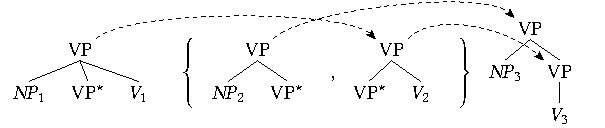
\includegraphics{graphics/abb515.pdf}
\caption{\label{fig-schema-231}TL-MCTAG-Derivation des String-Schemas $\mathit{NP}_2 ~ \mathit{NP}_3 ~ \mathit{NP}_1 $ $V_3$ $V_2 ~ V_1$}
\end{figure}

Im Geltungsbereich des SCC\is{Strong Co-occurrence Constraint (SCC)} kann TL-MCTAG\is{Multi-Component TAG (MCTAG)!baumlokale (TL-MCTAG)} jedoch nicht alle String"=Schemata aus $\scrind$ erzeugen. \citet[175]{Joshi:Becker:Rambow:00} behaupten, dass das beispielsweise bei folgendem String-Schema mit vier Verben der Fall ist:\footnote{Eine schöne vergleichende Darstellung der Ausdrucksstärke verschiedener TAG-Varianten bei vier Verben bieten übrigens \citet[Abbildung 3, Abbildung 7]{Chen-Main:Joshi:08} an. Dort werden auch weitere String-Schemata mit vier Verben aufgeführt, die für eine TL-MCTAG\is{Multi-Component TAG (MCTAG)!baumlokale (TL-MCTAG)} unter dem SCC\is{Strong Co-occurrence Constraint (SCC)} nicht derivierbar sind.}

\ex. $\mathit{NP}_2 ~ \mathit{NP}_4 ~ \mathit{NP}_3 ~ \mathit{NP}_1 ~ V_4 ~ V_3 ~ V_2 ~ V_1$\label{ex-schema-2431}

Hält man sich dagegen nur an das schwächere WCC\is{Weak Co-occurrence Constraint (WCC)}, so steht für \ref{ex-schema-2431} die TL-MC"-TAG-Ableitung in Abbildung~\ref{fig-schema-2431} zur Verfügung.
\begin{figure}[t]
\centering
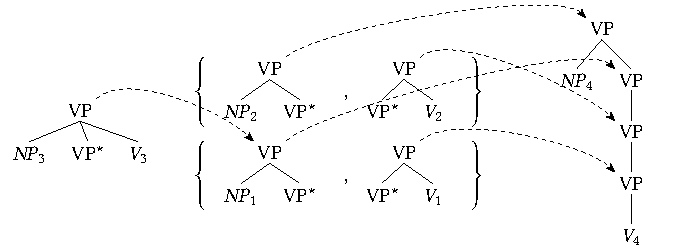
\includegraphics{graphics/abb516.pdf}
\caption{\label{fig-schema-2431}TL-MCTAG-Derivation des String-Schemas $\mathit{NP}_2 ~ \mathit{NP}_4 ~ \mathit{NP}_3$ $\mathit{NP}_1 ~ V_4 ~ V_3$ $V_2 ~ V_1$}
\end{figure}
Auf"|fällig an dieser TL-MCTAG ist der $V_4$-Ele\-men\-tarbaum mit den vier VP-Knoten, die dafür sorgen, dass die dargestellten Elementarbaummengen baumlokal verknüpft werden können. Wären weitere Elementarbaummengen involviert, müsste $V_4$ (oder ein anderer Elementarbaum) über eine entsprechende Anzahl zusätzlicher VP-Knoten verfügen, um alle Scramblingmöglichkeiten erzeugen zu können. Daran kann man sehen, dass es eine endliche TL-MCTAG\is{Multi-Component TAG (MCTAG)!baumlokale (TL-MCTAG)} für $\scrind$\is{indizierte Scramblingsprache ($\scrind$)} nicht geben kann: Je mehr Verben involviert sind, desto mehr Elementarbaummengen und desto mehr VP-Knoten in einem Elementarbaum müssen zur Verfügung stehen. Der Beweis in \cite{Becker:Rambow:Niv:92} zeigt zudem, dass $\scrind$ auch nicht durch eine mengenlokale MCTAG (SL-MCTAG)\is{Multi-Component TAG (MCTAG)!mengenlokale (SL-MCTAG)} derivierbar ist.\footnote{\label{fn-lcfrs} Genaugenommen zeigen \cite{Becker:Rambow:Niv:92}, dass $\scrind$ nicht durch eine LCFRS\is{Linear Context-Free Rewriting Systems (LCFRS)} generiert werden kann, und LCFRS enthält TL-MCTAG und SL-MCTAG. Siehe auch \citet[53ff]{Rambow:94}.} Was mit TL-MCTAG\is{Multi-Component TAG (MCTAG)!baumlokale (TL-MCTAG)} und SL-MCTAG allerdings derivierbar ist, ist etwas Eingeschränkteres, das man allgmein als $k$-$\scrind$\is{indizierte Scramblingsprache ($\scrind$)} aufschreiben kann:

\ex. $k$-$\scrind = \{ \sigma(\mathit{NP}_1,\ldots,\mathit{NP}_m) V_m \ldots V_1 | 1 \leq m \leq k$ und $\sigma$ ist eine Permuta"-tion$\}$

Während $k$ im Geltungsbereich des WCC\is{Weak Co-occurrence Constraint (WCC)} je Grammatik beliebig wählbar ist, gilt im Geltungsbereich des SCC\is{Strong Co-occurrence Constraint (SCC)} zumindest für TL-MCTAG\is{Multi-Component TAG (MCTAG)!baumlokale (TL-MCTAG)}: $k = 3$.

\cite{Joshi:Becker:Rambow:00} versuchen aus der mangelnden \isi{Ausdrucksstärke} eine Tugend zu machen und argumentieren, dass die Sprecherkompetenz\is{Kompetenz} nicht $\scrind$ enthält, sondern blo\ss\ 3-$\scrind$ und dass daher TL-MCTAG\is{Multi-Component TAG (MCTAG)!baumlokale (TL-MCTAG)} der richtige Kandidat für die Modellierung der Sprecherkompetenz darstellt.\footnote{\cite{Chen-Main:Joshi:08,Chen-Main:Joshi:12} führen diese Idee fort.} Diese Argumentation ist nicht unumstritten. Zum einen hält es \citet[Abschnitt~10.6.3]{Mueller:10} für möglich, das Sting-Schema $\mathit{NP}_2 ~ \mathit{NP}_4 ~ \mathit{NP}_3 ~ \mathit{NP}_1 ~ V_4 ~ V_3 ~ V_2 ~ V_1$ als grammatischen Satz zu instanziieren. Zwar fände man generell "`in Kopora keine Belege mit vier oder mehr eingebetteten Verben"' (S.~268) und die Verarbeitung der konstruierten Daten sei schwierig -- aber es sei keinesfalls unmöglich, wie \ref{ex-mueller-270-22} beweise:   

\ex. \label{ex-mueller-270-22}weil [der Frau]$_2$ [diesen Teich]$_4$ [den Mann]$_3$ niemand$_1$ leer$_4$ fischen$_3$ helfen$_2$ sah$_1$ \hfill \citep[270]{Mueller:10}

Der Satz sei durch Performanzfaktoren\is{Performanz} markiert und solle "`nicht von der Grammatik ausgeschlossen werden"'. Zum anderen moniert Müller, dass Umstellungen im TL-MCTAG-Modell mal kompetenzseitig und mal performanzseitig beschränkt sind, ohne dass dies durch die Umstellung selber gerechtfertigt wäre. Während beispielsweise \ref{ex-mueller-270-22} jenseits der Ausdrucksstärke von TL-MCTAG liegt, ist eine Umstellung wie in \ref{ex-mueller-270-21} durch eine TL-MCTAG adäquat modellierbar: 

\ex. \label{ex-mueller-270-21}weil niemand$_1$ [der Frau]$_2$ [diesen Teich]$_4$ [den Mann]$_3$ leer$_4$ fischen$_3$ helfen$_2$ sah$_1$ \hfill \citep[270]{Mueller:10}

Müller kann zwischen \ref{ex-mueller-270-22} und \ref{ex-mueller-270-21} keinen Markiertheitsunterschied feststellen, der es rechtfertigen würde, in dem einen Fall von einem Kompetenzphänomen\is{Kompetenz} und im anderen Fall von einem Performanzphänomen\is{Performanz} zu sprechen.\footnote{"`Ich halte es für falsch, Beschränkungen in Bezug auf Umstellbarkeit an der Mächtigkeit des Grammatikformalismus festzumachen, denn die Beschränkungen, die man finden kann, sind unabhängig von Verbalkomplexen bereits bei einfachen Verben mit zwei Argumenten wirksam."' \citep[269]{Mueller:10}} Wenn man zudem bedenkt, dass TL-MCTAG beliebig gro\ss e Verbalkomplexe erzeugen kann (die ja schon bei vier Verben schwer verständlich und nicht durch Korpora zu belegen sind), dann wirkt die durch TL-MCTAG definierte Performanz-Kompetenz-Schwelle reichlich willkürlich. %\\

Ob die mächtigste MCTAG-Variante nach \cite{Weir:88}, die nichtlokale MCTAG (NL-""MCTAG)\is{Multi-Component TAG (MCTAG)!nichtlokale (NL-MCTAG)}, $\scrind$\is{indizierte Scramblingsprache ($\scrind$)} derivieren kann, ist noch nicht abschlie\ss end geklärt, erscheint mir aber durch die geltende \isi{Simultanitätsbedingung} eher fraglich. Doch selbst wenn NL-MCTAG zu einer Derivierung von $\scrind$ in der Lage wäre, hätte die Modellierung mit NL-MCTAG\is{Multi-Component TAG (MCTAG)!nichtlokale (NL-MCTAG)} zwei Nachteile: Erstens ist seit \cite{Rambow:Satta:92} bekannt, dass NL-MCTAG unerwünschte Komplexitätseigenschaften besitzt. Zweitens erlaubt es NL-MCTAG trotzdem nicht, bestimmte Strukturvorstellungen in den Elementarbäumen umzusetzen. \citet[56f]{Rambow:94} identifiziert diese Unzulänglichkeit bei der Modellierung von Topikalisierungsdaten\is{Voranstellung} wie \ref{ex-schema2}, hier wiederholt als \ref{ex-schema2-1}:

\exg. {Dieses Buch} hat {den Kindern} niemand {zu geben} versucht.  \\
$\mathit{NP}_2$ $V_1$ $\mathit{NP}_2$ $\mathit{NP}_1$ $V_2$ $V_1$ \\
\citep[42]{Rambow:94} \label{ex-schema2-1}

Unter der Voraussetzung, dass \ref{ex-schema2-1} als Ergebnis einer \isi{Bewegung} von {\it dieses Buch} ("`long-distance topicalization"') und {\it den Kindern} ("`long-distance scrambling"') in den Matrixsatz modelliert werden soll, ergibt sich folgender Widerspruch:
Für eine Bewegungsanalyse sollte hier das eingebettete Infinitum {\it zu geben} und seine NP-Ergänzungen {\it dieses Buch} und {\it den Kindern} in unterschiedlichen Elementarbäumen einer Elementarbaummenge repräsentiert werden, damit die NP"=Ergänzungen im Baum des Matrixsatzes {\it hat niemand versucht} adjungieren.\footnote{Vgl.\ Abbildung~\ref{fig-mctag-bsp} auf Seite \pageref{fig-mctag-bsp}.} Gleichzeitig muss wegen des Valenzprinzips der regierende Matrixsatz {\it hat niemand versucht} irgendwie an {\it zu geben} adjungieren. Dies widerspricht jedoch der für NL-MCTAG\is{Multi-Component TAG (MCTAG)!nichtlokale (NL-MCTAG)} bestehenden \isi{Simultanitätsbedingung} bei der Anwendung einer Elementarbaummenge: Die Ergänzungen von {\it zu geben} müssen an etwas adjungieren, was (unmittelbar oder mittelbar) an {\it zu geben} adjungiert hat. Mit anderen Worten, selbst der Einsatz von NL-MCTAG\is{Multi-Component TAG (MCTAG)!nichtlokale (NL-MCTAG)} schränkt den Spielraum in der Gestaltung der Elementarstrukturen so ein, dass unangenehme Zugeständnisse nötig sind. Ein erstaunliches Ergebnis aus \cite{Rambow:94} ist da, dass sowohl die computationelle Komplexität als auch die Einschränkungen für die Grammatikimplementierung durch die Herausnahme der Simultanitätsbedingung wesentlich verbessert werden. Dazu mehr in Abschnitt~\ref{sec-tag-varianten}.
\is{Multi-Component TAG (MCTAG)|)}  


\subsection{Relativsatzextraposition und NP-PP-Splits} \label{sec-tag-grenzen-wellnest}

Andere Formen der \isi{Diskontinuität} mit je eigenen Grenzen für die TAG"=Modellierung liegen bei extraponierten Relativsätzen und NP-PP-Splits vor, auf die ich jedoch nur in diesem Abschnitt kurz eingehen möchte. %\\

\is{Satz!Relativ-|(}\is{Extraposition|(}
Die Beziehung zwischen Nomen und extraponiertem Relativsatz wird gemeinhin als syntaktische Beziehung aufgefasst und dementsprechend analysiert,\footnote{Eine Analyse als anaphorische Beziehung schlägt z.\,B.\ \cite{Kiss:05} vor.} etwa durch Basisgenerierung am Nomen und anschlie\ss ender Rechtsbewegung ins \isi{Nachfeld} \citep{Buering:Hartmann:97} oder mittels eines Slash-Mechanismus \citep{Pollard:Sag:94, Keller:95, Mueller:99}. Was das TAG-Framework betrifft, kommt der einschlägige Modellierungsvorschlag von \cite{Kroch:Joshi:87}, wobei sie eine TL-MCTAG\is{Multi-Component TAG (MCTAG)!baumlokale (TL-MCTAG)} verwenden und keine klassische TAG. Kroch und Joshi streben die Simulation einer Bewegungsanalyse\is{Bewegung} an und verwenden dafür Baummengen, die den extraponierten Relativsatz und seine Spur bündeln. Für die Extraposition in \ref{ex-kj87-70} schlagen sie daher die Baummenge in Abbildung~\ref{fig-kj87-1} vor: 

\ex. \label{ex-kj87-70} A man arrived who knew Mary. \hfill \citep[(70)]{Kroch:Joshi:87}

\begin{figure}[t]
\centering
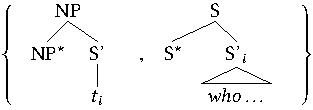
\includegraphics{graphics/abb517.pdf}
\caption{\label{fig-kj87-1}Elementarbaummenge für extraponierte Relativsätze gemä\ss\ \cite{Kroch:Joshi:87}}
\end{figure}
\largerpage%
Wenn man einen Elementarbaum für {\it arrived} annimmt, der dem Valenzprinzip gehorcht,\footnote{\citet[(71)]{Kroch:Joshi:87} zeigen nur einen bereits abgeleiteten Baum für {\it a man arrived}.} muss die Spur an dessen NP-Substitutionsknoten adjungieren und der Relativsatz an dessen S-Knoten. Die Baumlokalität garantiert dann die Einhaltung wichtiger Inselbeschränkungen.  

Sieht man von der Simulation einer Bewegungsanalyse ab, ist auch eine Modellierung ohne Baummengen, d.\,h.\ mit klassischer TAG, denkbar. In TAG werden Relativsätze wie Modifizierer durch Hilfsbäume repräsentiert, die an den Elementarbaum des modifizierten Nomens adjungieren. Das sollte auch für extraponierte Relativsätze gelten. Versucht man also für die Extraposition in \ref{ex-kj87-70} eine entsprechende TAG-Analyse zu finden, z.\,B.\ die stark vereinfachte in Abbildung~\ref{fig-extraposition-1}, dann stö\ss t man schnell auf Schwierigkeiten:\largerpage%  
\begin{figure}[t]
\centering
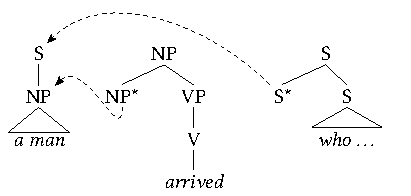
\includegraphics{graphics/abb518.pdf}
\caption{\label{fig-extraposition-1}Versuch einer TAG-Analyse für extraponierte Relativsätze}
\end{figure}
Zwar erfüllen die Elementarbäume das Valenzprinzip, aber der abgeleitete Baum genügt nicht dem Phrasenstrukturprinzip, weil nämlich darin ein S-Knoten nur einen NP-Knoten dominiert. Dies könnte noch ausgebessert werden, indem {\it arrived} an einem S-Knoten von {\it a man} adjungiert -- um den Preis freilich, dass {\it arrived} fälschlicherweise eine Satzkategorie subkategorisiert. 

Nun ist das hervorstechende Merkmal der Relativsatzextraposition deren potentielle Nichtlokalität, denn das Antezendens-Nomen kann beliebig tief in einem nominalen Satzglied eingebettet sein, wie in \ref{ex-extraposition} zu sehen ist:

\ex. \label{ex-extraposition}
\a. Karl hat mir das Bild einer Frau gegeben, die schon lange tot ist.
\b. Karl hat mir eine Fälschung des Bildes einer Frau gegeben, die schon lange tot ist.
\c. Karl hat mir eine Kopie einer Fälschung des Bildes einer Frau gegeben, die schon lange tot ist.
\z. \citep[(13.18)]{Mueller:99}

Au\ss erdem können mehrere Relativsätze von verschiedenen Ergänzungen und Angaben extraponiert werden.\footnote{Dank an Stefan Müller für den Hinweis!} \cite{Kroch:Joshi:87} gehen auf solche Extrapositionsdaten nicht ein und eine Modellierung mit TL-MCTAG\is{Multi-Component TAG (MCTAG)!baumlokale (TL-MCTAG)}, und daher auch mit TAG, scheint mir auch ausgeschlossen zu sein. Möglicherweise könnte man hier mit SL-MCTAG\is{Multi-Component TAG (MCTAG)!mengenlokale (SL-MCTAG)} noch etwas ausrichten.\is{Satz!Relativ-|)}\is{Extraposition|)} %\\


Ein ähnliches Problem stellen NP-PP-Splits wie in \ref{ex-npppsplit-1} dar:\is{NP-PP-Split|(}

\ex. \label{ex-npppsplit-1} Über Goethe las Peter ein Buch. 

Die Bestandteile des NP-PP-Splits, die NP {\it ein Buch} und die PP {\it über Goethe}, werden bisweilen (siehe etwa \citealt{DeKuthy:02}) als Bestandteile eines Valenzrahmens aufgefasst, worin {\it ein Buch} als Valenzträger und {\it über Goethe} als seine optionale Ergänzung fungieren. Darin liegt der Unterschied zur Relativsatzextraposition, bei der ein nominaler Valenzträger und seine  Angabe bzw.\ sein Modifizierer diskontinuierlich realisiert sind. Gemä\ss\ dem Valenzprinzip muss also im Elementarbaum von {\it ein Buch} die PP-Ergänzung {\it über Goethe} mittels nicht-terminalem Blatt angedeutet sein. Unter dieser Voraussetzung scheint eine TAG-Analyse von \ref{ex-npppsplit-1} zunächst möglich, z.\,B.\ mit den Elementarbäumen in Abbildung~\ref{fig-npppsplit-1}.
\begin{figure}[t]
\centering
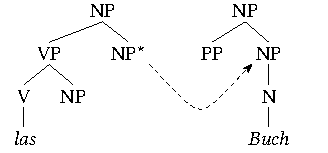
\includegraphics{graphics/abb519.pdf}
\caption{\label{fig-npppsplit-1}Versuch einer TAG-Analyse für NP-PP-Splits}
\end{figure}
Allerdings muss man dafür in Kauf nehmen, dass die resultierende Phrasenstruktur den Satz \ref{ex-npppsplit-1} als NP ausweist. Wie schon bei dem Modellierungsversuch einfachster Extrapositionsdaten (Abbildung~\ref{fig-extraposition-1}) kommt es also im günstigsten Fall zu falschen Kategoriezuweisungen, die mir unausweichlich erscheinen, da in beiden Fällen ein verbaler Valenzträger an eine nominale Ergänzung adjungieren muss. Andere Fälle von NP-PP-Split sind dagegen unerreichbar für eine TAG-Modellierung, z.\,B.\ die Konfiguration in \ref{ex-npppsplit-2}: 

\ex. \label{ex-npppsplit-2} Peter hat über Goethe an einem Tag zwei Bücher gelesen.

\largerpage%
Zur Veranschaulichung stelle man sich vor, dass Satz \ref{ex-npppsplit-2}  durch eine Adjunktion eines Hilfsbaums mit der Terminalkette  {\it Peter hat an einem Tag gelesen} an einen Elementarbaum mit der Terminalkette {\it über Goethe zwei Bücher} deriviert werden soll. Das ist jedoch unmöglich, weil die Terminalkette des Hilfsbaums (also {\it Peter hat an einem Tag gelesen}) bei der Adjunktion nur in maximal zwei Teile geteilt werden kann. In Satz \ref{ex-npppsplit-2} besteht sie aber aus drei Teilen. Ein analoges Problem trat bereits beim Scrambling in kohärenten Konstruktionen in \ref{ex-schema21} auf.
\largerpage% 

Dass auch die einfachsten Formen der Relativsatzextraposition\is{Satz!Relativ-}\is{Extraposition} und des NP-PP-Splits nicht immer  mit TAG modelliert werden können, sobald diese kombiniert werden, zeigt schlie\ss lich \ref{ex-kombination}:\footnote{Siehe auch die Diskussion in \cite{Chen-Main:Joshi:12}.}

\ex. \label{ex-kombination} Über Goethe las derjenige Schüler ein Buch, der als extrem lesefaul gilt. 

Beide Ergänzungen des Verbs {\it las} sind hier diskontinuierlich. Darüber hinaus überkreuzt sich aber der String des NP-PP-Splits mit dem String der Nominativ-NP {\it derjenige Schüler} und seines extraponierten Relativsatzes, so dass eine Adjunktion des Verbs nur eine der Diskontinuitäten erzeugen kann. Konfigurationen wie in \ref{ex-kombination} werden in der Dependenzliteratur als nicht-wohleingebettet\is{Non-well-nestedness} (non-well-nested / ill-nested) bezeichnet \citep{Bodirsky:etal:05}. \cite{Kuhlmann:Moehl:06} haben gezeigt, dass nicht-wohleingebettete Dependenzstrukturen\is{Dependenzgraph} nicht von einer LTAG induziert werden können. Dagegen sei dies mit TL-MCTAG\is{Multi-Component TAG (MCTAG)!baumlokale (TL-MCTAG)} prinzipiell möglich.
\is{NP-PP-Split|)}



\subsection{Ellipse}\is{Ellipse}

In Abschnitt \ref{sec-tag-ling} wurde festgestellt, dass ein TAG-Modell, dessen Elementarbäume dem $\theta$-Kriterium für TAG, dem PACP oder dem Valenzprinzip unterworfen sind, der Idealisierung der Vollständigkeit auf sehr konsequente Weise folgt: Elementarbäume, die einen Valenzrahmen repräsentieren, enthalten für alle obligatorischen Valenzrollen je ein nicht-terminales Blatt, das im Laufe der Derivation "`gefüllt"' werden muss. Elementarbäume mit phonetisch leerem Anker gelten als unlexikalisiert und stehen daher in einer lexikalisierten TAG nicht zur Verfügung. Die Weglassung obligatorischer Valenzrahmenbestandteile ist also ausgeschlossen. Wie wir in Kapitel~\ref{sec-ellipsenanalyse} sehen werden, gibt es für einen Teilbereich der Ellipsenphänomene Ansätze, diese sehr strikte Form der Valenzrealisierung zu umgehen. Dabei müssen allerdings erhebliche Abweichungen vom TAG-Formalismus in Kauf genommen werden. Das spricht vielleicht dafür, eine Korrektur der zugrundeliegenden Prinzipien in Betracht zu ziehen, nämlich das Valenzprinzip selber zu lockern oder Valenz sogar ganz von der Syntax zu entkoppeln. Darum wird es in Kapitel~\ref{ch-ohne-valenz} gehen. 

\section{Zusammenfassung}

In diesem Kapitel habe ich den TAG-Formalismus eingeführt und Anwendungsprinzipien für die Modellierung natürlicher Sprache erläutert. Elementarbäume werden demnach als komplexe syntaktische Repräsentationen interpretiert, deren Struktur und Knotenbeschriftungen maßgeblich durch die syntaktischen Eigenschaften der lexikalischen Anker determiniert sind. Diese Determinierung vollzieht sich entlang von Wohlgeformtheitsprinzipien, die in diesem Kapitel anhand von prominenten Explikationen, etwa dem CETM und dem $\theta$-Kriterium aus \cite{Frank:02}, dargestellt und diskutiert wurden. Weil sich die bisher vorgeschlagenen Explikationen als inadäquat erwiesen haben, wurden drei zentrale Wohlgeformtheitsprinzipien überarbeitet bzw.\ neu formuliert, nämlich das Phrasenstrukturprinzip, das Valenzprinzip und das Ökonomieprinzip. Für uns ist natürlich das Valenzprinzip von besonderem Interesse, weil es das Verhältnis zwischen Valenz und TAG-Syntax bestimmt. Schließlich bin ich auf die Grenzen der Ausdrucksstärke von TAG unter dem Einfluss dieser Wohlgeformtheitsprinzipien, insbesondere des Valenzprinzips, eingegangen. Die restlichen Kapitel werden sich u.\,a.\ damit befassen, wie diese zu engen Grenzen durch moderate Veränderungen am TAG-Formalismus geweitet werden können. 



